\documentclass[a4paper]{report}
\usepackage{setspace}
%\usepackage{subfigure}

\pagestyle{plain}
\usepackage{amssymb,graphicx,color}
\usepackage{amsfonts}
\usepackage{latexsym}
\usepackage{amsmath}
\usepackage{float}
\usepackage{rotating}
\usepackage[a4paper, margin = 3cm, bottom = 2.5cm]{geometry}
\usepackage{biblatex}
\addbibresource{bibliography.bib}

% Add autorefs with capitalized names (my preference)
\usepackage{hyperref}
\renewcommand{\chapterautorefname}{Chapter}
\renewcommand{\sectionautorefname}{Section}
\renewcommand{\subsectionautorefname}{Subsection}
\renewcommand{\subsubsectionautorefname}{Subsubsection}
\renewcommand{\figureautorefname}{Figure}
\renewcommand{\tableautorefname}{Table}

\newtheorem{theorem}{THEOREM}
\newtheorem{lemma}[theorem]{LEMMA}
\newtheorem{corollary}[theorem]{COROLLARY}
\newtheorem{proposition}[theorem]{PROPOSITION}
\newtheorem{remark}[theorem]{REMARK}
\newtheorem{definition}[theorem]{DEFINITION}
\newtheorem{fact}[theorem]{FACT}

\newtheorem{problem}[theorem]{PROBLEM}
\newtheorem{exercise}[theorem]{EXERCISE}
\def \set#1{\{#1\} }

\newenvironment{proof}{
PROOF:
\begin{quotation}}{
$\Box$ \end{quotation}}



\newcommand{\nats}{\mbox{\( \mathbb N \)}}
\newcommand{\rat}{\mbox{\(\mathbb Q\)}}
\newcommand{\rats}{\mbox{\(\mathbb Q\)}}
\newcommand{\reals}{\mbox{\(\mathbb R\)}}
\newcommand{\ints}{\mbox{\(\mathbb Z\)}}

%%%%%%%%%%%%%%%%%%%%%%%%%%


\title{{\vspace{-14em} 
\includegraphics[scale=0.4]{images/ucl_logo.png}}\\
{{\Huge GenAI and financial data alert systems}}\\
{\large GenAI Insight Overlays}\\
}
\date{Submission date: 8 September 2025}
\author{Candidate Number: KYHL7\thanks{
{\bf Disclaimer:}
This report is submitted as part requirement for the MSc. Computer Science at UCL. It is substantially the result of my own work except where explicitly indicated in the text. The report may be freely copied and distributed provided the source is explicitly acknowledged.}
\\ \\
MSc. Computer Science\\ \\
Internal Supervisor: Prof. Lewis D. Griffin}



\begin{document}
 
\onehalfspacing

\maketitle
\begin{abstract}
TODO: Summarise your report concisely.
\end{abstract}

\tableofcontents

\setcounter{page}{1}


\chapter{Introduction}
\label{chapter:introduction}

According to a study by Forrester Consulting, knowledge workers spend 30\% of their time --- that is, 2.4 hours a day --- searching for information within their own company\cite{forrester2022}. This is a significant amount of time that could be better spent making decisions and taking action. As such, the aim of this project is to explore the capabilities of Large Language Models (``LLMs") to access a company's data, extract operational figures and provide initial insights to managers, directly to their inbox, saving time from the operational task of data gathering, and allowing them to focus on the more impactful parts of their roles --- making data-informed decisions.

To perform this exploration, the goal is to creating a proof of concept system that acts as a junior analyst (or ``AI Analyst") who autonomously generates reports about a specific Key Performance Index (KPI), at set time intervals, based on the company's data. In addition to the AI Agent, the system will have a simple user interface, where the user can set the KPI(s) to report on, and the interval at which their analyst should run.

For this, the project builds on the recent evolution of AI agents and agentic systems, as paradigms that allow the execution of complex, multi-step workflows autonomously. Nevertheless, this specific use case poses a few challenges to the current stat of the art in GenAI agents.

For these reports, the AI Analyst must go beyond simply retrieving high-level KPIs. Instead, it must also provide granular details that uncover deeper operational insights. For example, rather than merely reporting that sales are down by 10\%, the Analyst should also identify which products or regions are driving this decline.

This type of work is inherently open-ended. There is no single ``correct" answer, or even path to an answer, nor a clear point to stop, and the AI Analyst must adapt its approach depending on its own intermediate findings. Crucially, for the reports to be truly useful, the agent must not just report the data, but drawing causal inferences that can point the manager in the right direction to solve any issues found, something that remains a known challenge for LLMs \cite{llmcausalreasoning2024}.

Moreover, this kind of internal analysis is not likely to be included in LLM's training sets. Companies rarely publish their internal data or reports, and the requirements of operational reports are more granular than financial reports, which might be available for public companies. This makes the task a strong candidate for fine-tuning, but due to the lack of suitable training data this is outside of the project scope.

With all of this in mind, the project was executed in three consecutive stages: First, a Research stage, focused on understanding the state of the art in AI agent orchestration and prompting, as well as the software tools available; the results of this stage can be found in \autoref{chapter:research}. Second, a Requirements and Analysis stage, where together with the client, Alvarez \& Marsal, we defined the scope of the proof of concept; the results of this stage can be found on \autoref{chapter:requirements-analysis}. This was also the bases for the evaluation framework for the project, which is described in \autoref{chapter:evaluation-testing}. Third, a Design and Implementation stage, which was performed iteratively; the details of this stage can be found on \autoref{chapter:design-implementation}. Finally, \autoref{chapter:reflections} contains the Reflections from the process of creating the proof of concept system, as well as the potential future work to create a production-ready system.

\chapter{Research}
\label{chapter:research}

Research for this project was be split in two main lines. First, understanding the fundamentals of building applications with Large Language Models. For this, the project was largely influenced by Chip Huyen's book, AI Engineering, which ``provides a framework for adapting foundation models, which include both large language models (LLMs) and large multimodal models (LMMs), to specific applications"\cite{aiebook2025}. In particular, a few learnings from the book were crucial in the development stage, which give structure to \autoref{sec:research-llms}:

\begin{enumerate}
    \item Its highlight of the importance, and difficulty, of evaluating AI systems
    \item Its guideline of Prompt Engineering best practices
    \item Its guideline of Retrieval Augmented Generation
    \item Its overview of AI Agents
\end{enumerate}

That said, this chapter does not intend to replicate the book's content, instead it will describe the most important learnings grasped from it, and add the learnings from other relevant information sources.

Afterwards, \autoref{sec:research-tools} will describe the research performed to define the technology stack used to develop the proof of concept, which per the client's request was built in a python environment.

\section{Large Language Models and Agents Learnings}
\label{sec:research-llms}

\subsection{AI System Evaluation}

In AI Engineering, Chip Huyen highlights two main reasons why evaluating the outputs of LLMs is harder than evaluating traditional machine learning models.

First, as tasks become more sophisticated, the more time it takes to evaluate them. As she puts it, ``[y]ou can  no longer evaluate a response based on how it sounds. You'll also need to fact-check, reason, and even incorporate domain expertise".  Secondly, the open-ended and probabilistic nature of LLMs "undermines the traditional approach of evaluating a model against ground truths". There are too many correct responses, so it is impossible to have a comprehensive list of correct outputs as ground truth.

These problems are exacerbated when it comes to AI Agents, as they tackle more complex tasks. This is an on-going research field but, according to \cite{krishnan2025aiagentsevolutionarchitecture}, the focus of evaluation so far has been ``predominantly focused on accuracy metrics that measure task completion success". This focus has been criticised for many reasons, particularly for limiting the evaluation to a task being completed or not, and not included other metrics such as the efficiency of the completion.

This type of measure is called ``exact evaluation'', because it has no ambiguity --- a task is complete or it is not --- and can be viewed more generally to include any type of rules-based evaluation where, as the name indicates, a set or rules are defined and the output is measured against it adherence to these rules.

The alternatives to this type of evaluation are what has been called ``objective evaluations'', where an external validator that reviews the agent's output and ``judges'' it, assigning it a score based on some type of defined criteria --- for example completeness or clarity. So far, studies such as \cite{wang2025replacehumanevaluators} have found that this judgment can be performed by either LLMs (LLM as a judge) or Humans (Human as a judge), with high correlations in the scores given. Nevertheless, \cite{hu2023decipher} has also found that human's personal preferences can affect the score given to an output.

Moreover, other authors such as \cite{zhuge2024agentasajudgeevaluateagentsagents} criticize any approach for evaluating Agents that relies solely on the final output of their process. They believe that agents shouldn't only be evaluated on their final output but on the intermediate steps taken, and thus propose agent as a judge -a methodology that uses agents to enable intermediate feedback- as a better alternative.

Evidently, despite the lack of a clear ``best" strategy, evaluation remains a key ingredient in creating AI systems to ensure their reliability. The AI Engineering book goes as far as proposing a development methodology called Evaluation Driven Design (EDD). Similarly to Test Driven Design, in EDD the evaluation criteria for the application are defined before building the application, allowing safe iterations. Moreover, her recommendations align with \cite{zhuge2024agentasajudgeevaluateagentsagents} in the need to not only evaluate the final output, but also every component of the system. As will be discussed in detail in \autoref{chapter:evaluation-testing}, this project followed the book's recommendations.

But how do you define said evaluation criteria? Huyen proposes thinking in three categories which, despite being targeted for evaluating LLMs and not agents, can be adapted as follows:

\begin{itemize}
    \item Domain-Specific Capacity: Evaluate the ability of the agent to perform tasks specific to the problem domain, such as coding or finance.
    \item Generation Capacity: Evaluate the quality of the text being generated, including the factual consistency of the outputs (that is, that the facts in the response are correct).
    \item Instruction-Following Capacity: Evaluate how well the specific instructions of a prompt are followed.
\end{itemize}

\subsubsection{Choosing the Right Model}

The difficulty in evaluation of LLMs and Agents highlights one specific buy key issue --- how do you choose the right model, or at the very least model family, to power an agent?

The literature points towards using specialized model for tasks that require domain specific capabilities, such as data analysis, and more general models for task that are common in the general training data, such as coding, tool calling or general summarization (e.g., writing the final report). Studies such as \cite{ke2025demystifyingdomainadaptiveposttrainingfinancial} and \cite{tanabe2024enhancingfinancialdomainadaptation} have shown that smaller models specifically trained for financial tasks outperform larger models in financial benchmarks.

Nevertheless, \cite{lu2025bizfinbench} created a financial benchmark that includes finance specific tasks such as forecasting market trends, predict asset movements, or analysing causal relationships in financial events, which closely resemble the types of task required in this project. Their evaluations of general models such as OpenAI's GTP-4o or o4-mini produced strong results (above 80\%) for these tasks, and as-such, these are used for development in this project. This is in line with the client's preferences of using widely available models.

\subsection{Prompt and Context Engineering}

According to Chip Huyen, ``[a] prompt is an instruction given to a model to perform a task''. One of the main reasons to build an evaluation framework is to be able to perform Prompt Engineering, or the process of tweaking prompts and context to get the desired outcome from an LLM. This step is so important, that model providers often provide detailed guides on how to engineer prompts for their specific models, such as \cite{openai2025promptengineering} from OpenAI, which guided the promp engineering process for this project. Most of guides, nonetheless, include two techniques that have become cornerstones for this process.

First is ``few-shot'' prompting, introduced by \cite{brown2020languagemodelsfewshotlearners}. This paper, by Brown et al., demonstrated that language models can learn a desired behaviour from examples in within the prompt; in more colloquial terms, there is a benefit to providing examples in prompts.

Second, there is ``Chain-of-Thought'' prompting, introduced by \cite{wei2023chainofthoughtpromptingelicitsreasoning}. In this type of prompt, the model is asked to perform a step by step process before providing an output --- either steps pre-defined in the prompt or defined by the model during execution. Wei et al. where able to achieve state of the art results using this technique.

Note that these techniques are not mutually exclusive, and prompts for complex tasks might include both of them, or none, depending on the specific model used (e.g., reasoning models might not need explicit chain of thought prompting).

\subsubsection{Context Engineering}

Borrowing AI Engineering's definition, the context is ``the information provided to the model so that it can perform a given task''. While the instruction (Prompt) remains static for any query, the information (Context) varies.

One key pattern for context engineering is Retrieval Augmented Generation (RAG), which according to AI Engineering can be considered as "a technique to construct context specific to each query". The pattern of retrieving and then generating was first introduced by Chen et al. in \cite{chen2017readingwikipediaansweropendomain}, where their system would retrieve Wikipedia pages relevant to a question and add their content to a model's context, and then fully coined by \cite{lewis2021retrievalaugmentedgeneration}.

While these two papers define the technique with the use of text, this pattern can be applied to any type of information. Most relevant to this project, tabular data can also be retrieved and provided as part of the context.

Finally, adding information is not the only way to manage a task's context. In perhaps the most important finding for this project, \cite{veseli2025positionalbiasesshiftinputs} demonstrates that as the size of the context grows closer to the model's limit, retrieval and reasoning become more biased towards data that is near the end of the context, and the model more easily fails to retrieve information provided in previous parts of the context.

\subsection{Agent Architectures and Agentic Orchestration}

According to \cite{sapkota2025aiagentsvsagentic}, ``AI Agents can be defined as autonomous software entities engineered for goal-directed task execution within bounded digital environments'', usually with an LLM as their ``core reasoning component''. They distinguish AI Agents from Agentic AI, an ``emerging class of systems [that] extends the capabilities of traditional AI Agents by enabling multiple intelligent entities to collaboratively pursue goals through structured communication, shared memory, and dynamic role assignment''. This subsection summarizes research findings for state of the art architectures of both.

\subsubsection{Agent Architecture}

The basic structure of an agent is described in AI Engineering as an LLM, which can perform certain actions (through tools) in a defined environment. The LLM acts as the brain of this agent, processing the information it receives --- e.g., the task given by the user or results from its own tools --- and generating plans to perform the task.

The plans designed by the LLM can be performed in many ways, for example, tools can be called in parallel or sequentially, or the LLM and tools call be called in a Loop until the LLM itself decides the task has been completed. This designed is generally called the Agent's Architecture.

One of the key problems for any Agent Architecture is how to build in ways to adjust the plans laid out by the LLM, allowing them to correct potential errors. On this, one of the most common patterns is ReAct (Reasoning and Acting), proposed by \cite{yao2023react}. In this pattern, two steps are taken in a loop until the task is completed: a Reasoning step, which encompass both planning and reflecting on tool outputs, and an Action step, where the next step in the plan is executed.

This architecture was later expanded upon in \cite{shinn2023reflexion}, in their proposed Reflexion architecture. In Reflexion, the agent has separate steps for evaluating the output of its tools and self-relect on what went wrong, on each iteration, after evaluation and reflection, the agent proposes a new plan, and then executes the next step on that plan.

\subsubsection{Agentic Orchestration Architecture}

As described by \cite{sapkota2025aiagentsvsagentic}, Agentic AI allows multiple AI Agents to collaborate for more complex goals. Agentic Orchestration thus refers to the way that the collaboration between agents is structured.

There are numerous ways to structure this collaboration. Some of the best known are, as described as part of LangGraph's documentation in \cite{langgraphagmultiagentsystems}, Networks (or Swarms) --- where all agents communicate in a single group --- and Supervisor --- where an LLM acts as the coordinating node. But there are numerous ways of coordinating the work across agents, according to a specific task needs.

For instance, in \cite{fourney2024magenticone}, a team of Microsoft researchers described Magentic-One, a generalist system that demonstrated state of the art performance in multiple agentic benchmarks without changing how the agents collaborate. The architecture is described by them as ``a multi-agent architecture where a lead agent, the Orchestrator, plans, tracks progress, and re-plans to recover from errors. [...] Moreover, Magentic-One's modular design allows agents to be added or removed from the team without additional prompt tuning or training, easing development and making it extensible to future scenarios''.

One of the most interesting parts about Magentic-One is that it applies the learnings from \cite{shinn2023reflexion} to multi-agent orchestration, that is, it has explicit steps to evaluate  outputs, analyze what went wrong and re-plan. The architecture was open sourced by Microsoft and, for these reasons, was used extensively in this project for its generalist capabilities.

\section{Software Tools}
\label{sec:research-tools}

While the project involved numerous decisions about tools, such as libraries to use for certain tasks, or the type of database to use to store user preferences, this section will only detail the key decisions that had an system-architecture impact: the frameworks used for user interface and agent orchestration, and the tool to schedule agent runs. They will be presented in this chapter in order of importance.

An important note is that the client had a preference for using Azure/Microsoft products for any infrastructure requirements, due to its enterprise readiness. Azure was thus used as inference provider (i.e., LLMs calls are performed through Azure AI Foundry). The client could not provide access to their own instances though, so the Azure student subscription was used independently of some of its limitations in model access and rate limiting.

\subsection{Agent Orchestration Frameworks}

Selecting the appropriate orchestration framework was the most crucial decision for the project, and the key guiding point for this was the size of a framework's community, which is often indicated by the number of GitHub stars. Community size can significantly influence the availability of resources such as documentation, tutorials, and community support. A larger community typically leads to more comprehensive examples and a broader base of shared knowledge, facilitating smoother development and troubleshooting processes.

As such, \autoref{tab:orchestration_frameworks_stars} compares several prominent Python frameworks for agentic orchestration, highlighting their community size and the implications for developers seeking robust support and resources.

\begin{table}[h]
\centering
\begin{tabular}{|p{3cm}|p{3cm}|p{9cm}|}
    \hline
    \textbf{Framework} & \textbf{GitHub Stars} & \textbf{Community Notes} \\ \hline
    \textbf{LangChain / LangGraph} & 113.6k & Extensive tutorials, active forums, and a wide array of integrations. \\ \hline
    \textbf{AutoGen} & 43.1k & Used to have support from Microsoft, with growing number of examples, but currently in the process of being merged to Semantic Kernel. \\ \hline
    \textbf{OpenAI SDK} & 8.6k & Official OpenAI support, with increasing community contributions. \\ \hline
    \textbf{CrewAI} & 35.8k & Active development with a focus on multi-agent collaboration. \\ \hline
    \textbf{Semantic Kernel} & 25.8k & Backed by Microsoft, offering enterprise-grade features, but documentation focused on C\#. \\ \hline
\end{tabular}
\caption{Comparison of Python Agentic Orchestration Frameworks}
\label{tab:orchestration_frameworks_stars}
\end{table}

Additionally, the \autoref{tab:orchestration_frameworks_uses} provides some findings on the same frameworks' functionality, ideal use cases, and the pros and cons associated with each.

\begin{table}[h]
\centering
\begin{tabular}{|p{3cm}|p{3cm}|p{3cm}|p{5.5cm}|}
    \hline
    \textbf{Framework} & \textbf{Functionality} & \textbf{Use Cases} & \textbf{Pros and Cons} \\ \hline
    \textbf{LangChain / LangGraph} & Modular pipeline for LLMs, embeddings, tools & Complex workflows, data pipelines & Pros: Extensive integrations, strong community support; Cons: Steep learning curve, large framework size \\ \hline
    \textbf{AutoGen} & Multi-agent orchestration with conversational agents & Multi-agent systems, collaborative tasks & Pros: Easy to implement multi-agent system, original implementation of Magentic-One; Cons: In process of being merged to Semantic Kernel \\ \hline
    \textbf{OpenAI Agents SDK} & Lightweight framework with agents, handoffs, and guardrails & Rapid prototyping, simple agent workflows & Pros: Minimal abstractions, easy to learn; Cons: Heavily geared towards using the full OpenAI ecosystem \\ \hline
    \textbf{CrewAI} & Role-based collaboration with task management & Team-based workflows, sequential tasks & Pros: Intuitive design, good for structured workflows; Cons: Less flexibility for complex scenarios, smaller community \\ \hline
    \textbf{Semantic Kernel} & Enterprise-grade framework & Enterprise applications, integration with Microsoft tools & Pros: Strong enterprise support, robust features, includes a default implementation of Magentic-One; Cons: Limited Python support, smaller community \\ \hline
\end{tabular}
\caption{Comparison of Python Agentic Orchestration Frameworks}
\label{tab:orchestration_frameworks_uses}
\end{table}

As will be explained in more detail later, the development of the project consisted of two iterations. The first iteration tried to take advantage of Microsoft's Magentic-One orchestration architecture, and that, in combination with the use of Azure as inference provider, made it an easy choice to use Semantic Kernel. On the contrary, the second iteration's approach is to build a detailed workflow with careful management of the data used in context, thus making LangChain/LangGraph a better fit, not just for its functionality but for the amount of documentation and examples available to support building this more detailed workflow.

\subsection{Scheduling Tool}

The project requires the AI agent to run at set intervals, as defined by the user preferences. Two primary scheduling alternatives were considered: Celery and cron (through the python crontab library).

Celery is a distributed task queue that supports asynchronous and real-time task execution, with advanced features such as retries, task prioritization, and integration with message brokers like Redis or RabbitMQ. While powerful, Celery introduces additional system complexity and overhead, requiring configuration of worker processes and a message broker.

In contrast, cron is a native, time-based scheduler available on Unix-like systems, designed specifically for executing tasks at fixed intervals. Cron is straightforward to configure, persistent across system reboots, and does not require any additional services.

Given the project's scope as a proof of concept, and the requirement of periodic execution at set intervals, cron was selected as the more practical solution.

\subsection{User Interface Framework}

Finally, for setting up the configuration interface, several Python frontend options were considered. The main alternatives evaluated were Streamlit, Gradio, and FastAPI with Jinja2 templates. While Streamlit and Gradio offer very quick setup and ease of use for prototypes, FastAPI with Jinja2 was chosen for this project due to its high customizability and the ability to easily scale the prototype into a full production application if needed.

\begin{table}[h]
\centering
\begin{tabular}{|p{2.5cm}|p{4cm}|p{4cm}|p{4cm}|}
\hline
\textbf{Feature \rule{0pt}{0.5cm}} & 
\textbf{Streamlit \rule{0pt}{0.5cm}} & 
\textbf{Gradio \rule{0pt}{0.5cm}} & 
\textbf{FastAPI + Jinja2 \rule{0pt}{0.5cm}} \\ \hline
\textbf{Primary Use Case} & Interactive dashboards & ML model interfaces & API-driven web apps \\ \hline
\textbf{Ease of Setup} & Very easy; minimal code & Very easy; minimal code & Moderate; requires setup \\ \hline
\textbf{Customization} & Limited UI customization & Limited UI customization & High; full control \\ \hline
\textbf{Performance} & Moderate & Moderate & High; asynchronous support \\ \hline
\textbf{Extensibility} & Limited & Limited & High; supports plugins \\ \hline
\textbf{Recommended Deployment} & Streamlit Cloud & Gradio Hub & Flexible (e.g., Docker, Cloud) \\ \hline
\textbf{Best For} & Rapid prototyping & Quick ML demos & Scalable, production-ready apps \\ \hline
\end{tabular}
\caption{Comparison of Python Frontend Frameworks for AI Agent Configuration}
\label{tab:framework_comparison}
\end{table}

\chapter{Requirements and Analysis}
\label{chapter:requirements-analysis}

As mentioned before, the client for this project is Alvarez \& Marsal (A\&M), a global professional services firm specializing in turnaround management, corporate restructuring, and performance improvement.

A\&M clearly identified a problem to solve: Executives spend valuable hours navigating dashboards just to extract the specific information relevant to their needs. As such, they wanted to explore the capabilities of LLMs to help reduce this time by building an Agentic AI system that could access a company's data, extract operational figures and generate report about a specific KPI, delivered directly to a user's email. For this, A\&M shared bullet points with their ideal set of functionalities for the system.

Nevertheless, as a professional services firm, Alvarez \& Marsal was limited in the resources they could share for the development of the system. Particularly, they were not allowed to provide anonymized data, which severely limited the functionalities that could be built --- as an example, while they wanted the system to retrieve news that could explain a reduction in sales, this only makes sense if the system knows which products the company is selling.

Due to this limitation, it was agreed to build a proof of concept system that could later be extended by their internal team. This chapter thus details the process for arriving to the requirements for this proof of concept system. First, the creation of user personas, and their scenarios for using the system, to help narrow the key need for users. Second, the definition of a set of requirements based on said personas.

Readers will note that this process did not include the definition of Use Cases. This is intentional, as the system has a single use case --- a user setting the report they want to receive, and when they want to receive it. Other than that, the system is autonomous.

\section{User Personas and Scenarios}

A\&M identified 2 types of users they wanted to target, based on their experience advising companies: a Sales Manager and a CFO-level user. The following are Fictional Personas, as well as a set of user scenarios where the system could improve their day to day work. The process of creating these drew heavily from \cite{ixdf_personas_2025} and \cite{ixdf_user_scenarios_2025}, and was based both on A\&M and the author's experience in industry.

\subsubsection{John, the Sales Manager}

\begin{tabular}{|p{3.3cm}|p{10.5cm}|}
\hline
\textbf{Hard Facts} & John lives in London, is 30--35 years old, and works as the Sales Manager for Germany for a car parts manufacturer. \\
\hline
\textbf{Computer and Internet Use} & He mainly uses a computer for work, including emails, reviewing dashboards, and browsing the internet for news and social media. He also owns an iPad and a MacBook. He is comfortable with computers but isn't particularly tech-savvy. \\
\hline
\textbf{A Typical Monday} & John starts his work week by reviewing unread emails to set priorities. He can spend up to two hours reviewing the company's dashboard to track sales in Germany. He then schedules follow-up meetings and spends the afternoon in meetings with his team and clients. \\
\hline
\textbf{Current Scenarios (As is)} & 
\begin{minipage}[t]{\linewidth}
    \begin{itemize}
        \item \textbf{All good}: John navigates the dashboard to see that sales are on track and he can move on with his day.
        \item \textbf{Issue found}: John notices a sales decline, investigates by manually filtering through different views (clients, number of active clients, churned clients), and then works with his team to create an action plan.
        \item \textbf{Continue what's working}: John sees a better-than-expected sales increase, investigates by looking at top clients and specific products, and then finds a news article about a change in safety regulations that might be driving the trend. He then advises his team to review the regulation and try to up-sell more customers.
    \end{itemize}
    \vspace{0.05em}
\end{minipage} \\
\hline
\textbf{Future Scenarios (To be)} & 
\begin{minipage}[t]{\linewidth}
    \begin{itemize}
        \item \textbf{All good}: John receives an email with a short report showing sales are on target, skims it, and moves on with his day.
        \item \textbf{Issue found}: John receives an email with a report attached that notes a sales decline and lists the clients who have churned, allowing him to forward the report and schedule a meeting with his team.
        \item \textbf{Continue what's working}: John receives an email with a report pointing out a higher-than-expected increase in sales for a specific product and links to a news article about a change in safety regulations, enabling him to forward the report and advise his team.
    \end{itemize}
    \vspace{0.05em}
\end{minipage} \\
\hline
\end{tabular}


\subsubsection{Clara, the CFO}

\begin{tabular}{|p{3.3cm}|p{10.5cm}|}
\hline
\textbf{Hard Facts} & Clara lives in Cambridge with her family, is 45--50 years old, and works as the CFO of John's company. \\
\hline
\textbf{Computer and Internet Use} & She mainly uses a computer for work, including emails, reviewing dashboards, and browsing the internet. She is "definitely not a tech-savvy person." \\
\hline
\textbf{A Typical Monday} & Clara starts her week by reviewing emails and spends up to an hour reviewing the company's dashboard to identify high-level trends. She has lunch with the CEO to discuss strategic planning and spends the afternoon in meetings with her team. \\
\hline
\textbf{Current Scenarios (As is)} & 
\begin{minipage}[t]{\linewidth}
    \begin{itemize}
        \item \textbf{All good}: Clara navigates through different dashboard screens to check various KPIs and finds they are all on track.
        \item \textbf{Issue found}: Clara notices a decline in Gross Margin, investigates by looking at sales and costs, and finds an unexpected cost increase in France, which she then notes and instructs her team to investigate.
        \item \textbf{Continue what's working}: Clara sees a positive increase in sales growth, investigates by looking at business lines, and finds an uptick in the Brakes division. She then looks for news, finds a regulation change in Germany, and schedules a meeting with the corresponding sales team to strategize.
    \end{itemize}
    \vspace{0.05em}
\end{minipage} \\
\hline
\textbf{Future Scenarios (To be)} & 
\begin{minipage}[t]{\linewidth}
    \begin{itemize}
        \item \textbf{All good}: Clara receives an email with a short report on all the KPIs she monitors, skims it, and moves on.
        \item \textbf{Issue found}: Clara receives an email with a report mentioning a KPI (Gross Margin) decline and a detailed explanation of the cause (increased costs in the France unit), allowing her to instruct her team to investigate immediately.
        \item \textbf{Continue what's working}: Clara receives an email with a report that points out an increase in sales for the Brakes product group and links to a news article about the related safety regulation change in Germany. This allows her to schedule a meeting with the corresponding sales team to discuss the impact and prepare for similar changes in other countries.
    \end{itemize}
    \vspace{0.05em}
\end{minipage} \\
\hline
\end{tabular}

\subsection{Analysis}

As put by \cite{ixdf_personas_2025}, Fictional Personas are deeply flawed. Nevertheless, they can be used as initial sketches of user needs. Based on these two particular user personas, a few things are important to drive adoption of any solution:

\begin{enumerate}
    \item \textbf{User interface needs to be easy to use:}
    \begin{itemize}
        \item Target personas are not particularly tech savvy.
        \item They are used to the intuitive interface of dashboards.
        \item They don’t want to spend 5 hours setting something up that only saves them a few hours per month—they want to spend 5 minutes.
        \item The key output they need is knowing where to look in detail for their next steps, so a high-level report can be good enough.
    \end{itemize}

    \item \textbf{Our users target a different number of KPIs, and this affects the level of detail they want to see:}
    \begin{itemize}
        \item A Sales Manager tracks a single KPI (Sales), but they want to go into a loot of operational detail. A CFO, on the other side, follows multiple high-level KPIs, but only wants to have a general understanding of the situation.
        \item Moreover, our target personas are used to being able to see exactly the level of operational detail they want from their dashboards. The system must be aware of that level of detail.
    \end{itemize}
    \item \textbf{Our users want a quick way of knowing if they need to review the report in detail:}
    \begin{itemize}
        \item This can be addressed in two ways. First, the report must contain an Executive Summary. Second, the email for the report should include the key findings.
    \end{itemize}
\end{enumerate}

\section{MoSCoW Requirements}

% Define counters
\newcounter{frcounter}
\newcounter{nfrcounter}

% Formatting for IDs
\newcommand{\frid}{FR-\arabic{frcounter}}
\newcommand{\nfrid}{NFR-\arabic{nfrcounter}}

Based on the user personas, and the limitations on data availability, the following requirements were defined for the system. Nevertheless, before reviewing them in detail there are a few important things to note.

First, as noted in the analysis of User Personas, the level of detail of the reports for the two types of personas are different --- in practical terms, this means the prompts that are used for one type of user might not work for the other. As such, it was decided to split certain requirements related to the report content by type of users.

Second, due to the nature of this project as a proof of concept, and due to the limitations in data availability mentioned before, the system will only implement a subset of all potential requirements. However, knowing what requirements might be implemented in the future can inform design decisions in the present. As such, it was deemed acceptable to have a long list of Won't Have requirements --- that is, a long list of requirements that are known and wanted for the system, but that will be outside of the scope of this project.

Finally, due to the limitations on data availability, it was decided that the proof of concept would only cover Sales Manager users. While A\&M could anonymize sales data with relative speed \footnote{This speed came with a cost though, as you will notice if you review the sample report, there are some drastic fluctuations in sales that can only be explained by issues with this process.}, the time needed to anonymize enough data for other KPIs was deemed too long for the project.

With this in mind, the following tables reflect the requirements for the project's system.
\subsection{Functional Requirements}

\subsubsection{Sales Manager}

\begin{tabular}{|l|p{10cm}|l|}
\hline
\textbf{ID} & \textbf{Requirement} & \textbf{Priority} \\
\hline
\stepcounter{frcounter}\frid & The system shall allow a Sales Manager-type user to set up their Sales scope (e.g., a specific region or product) & Must Have \\ \hline
\stepcounter{frcounter}\frid & The system shall be able to generate a Sales performance report based on the user’s preferences & Must Have \\ \hline
\stepcounter{frcounter}\frid & The system shall be able to identify “special cases” in Sales trends and perform a deeper analysis & Must Have \\ \hline
\stepcounter{frcounter}\frid & The system shall be able to provide simple Sales forecasts based on current trends & Should Have \\ \hline
\stepcounter{frcounter}\frid & The system shall be able to recommend potential actions to remedy “special cases” in Sales trends & Should Have \\ \hline
\stepcounter{frcounter}\frid & The system shall be able to provide simple Sales forecasts based on the remedy actions recommended by itself & Could Have \\ \hline
\stepcounter{frcounter}\frid & The system shall be able to provide advanced Sales forecasts using regression techniques or any other statistical method & Won’t Have \\
\hline
\end{tabular}

\subsubsection{CFO}

\begin{tabular}{|l|p{10cm}|l|}
\hline
\textbf{ID} & \textbf{Requirement} & \textbf{Priority} \\
\hline
\stepcounter{frcounter}\frid & The system shall allow a CFO-type user to set up a list of KPIs they follow & Won’t Have \\ \hline
\stepcounter{frcounter}\frid & The system shall be able to generate a report for the user’s KPI list & Won’t Have \\ \hline
\stepcounter{frcounter}\frid & The system shall be able to provide simple forecasts for each KPI based on current trends & Won’t Have \\ \hline
\stepcounter{frcounter}\frid & The system shall be able to identify “special cases” in the trend of any KPI and perform a deeper analysis & Won’t Have \\ \hline
\stepcounter{frcounter}\frid & The system shall be able to recommend potential actions to remedy “special cases” in each KPI’s trend & Won’t Have \\ \hline
\stepcounter{frcounter}\frid & The system shall be able to provide simple forecasts for each KPI based on the remedy actions recommended by itself & Won’t Have \\ \hline
\stepcounter{frcounter}\frid & The system shall be able to provide advanced forecasts for each KPI using regression techniques or any other statistical method & Won’t Have \\
\hline
\end{tabular}

\subsubsection{User Type Independent Requirements}

\begin{tabular}{|l|p{10cm}|l|}
\hline
\textbf{ID} & \textbf{Requirement} & \textbf{Priority} \\
\hline
\stepcounter{frcounter}\frid & The system shall email the resulting report to the email addresses configured by the user & Must Have \\ \hline
\stepcounter{frcounter}\frid & The system shall customize the email with the key findings of the report & Should Have \\ \hline
\stepcounter{frcounter}\frid & The system shall include both financial and operational information in a report & Must Have \\ \hline
\stepcounter{frcounter}\frid & The system shall be able to load information from a CSV file & Must Have \\ \hline
\stepcounter{frcounter}\frid & The system shall be able to load information from other files provided by the user & Won't Have \\ \hline
\stepcounter{frcounter}\frid & The system shall be able to load information from a set of reliable online information sources & Won't Have \\ \hline
\end{tabular}

\subsection{Non-Functional Requirements}

\begin{tabular}{|l|p{10cm}|l|}
\hline
\textbf{ID} & \textbf{Requirement} & \textbf{Priority} \\
\hline
\stepcounter{nfrcounter}\nfrid & The system shall be extensible to other sources of information & Must Have \\ \hline
\stepcounter{nfrcounter}\nfrid & The system shall run autonomously at fixed intervals & Must Have \\ \hline
\stepcounter{nfrcounter}\nfrid & The system shall allow the user to update the fixed interval for runs & Must Have \\ \hline
\stepcounter{nfrcounter}\nfrid & The system shall provide a user interface to update its configuration & Should Have \\ \hline
\stepcounter{nfrcounter}\nfrid & The system shall provide a user interface that is clear and easy to use & Should Have \\ \hline
\stepcounter{nfrcounter}\nfrid & The system shall allow multiple users to set up their reports & Could Have \\ \hline
\stepcounter{nfrcounter}\nfrid & The system shall allow users to authenticate before updating their report preferences & Won’t Have \\ \hline
\end{tabular}

\chapter{Design and Implementation}
\label{chapter:design-implementation}

NOTE: Talk about the experiments here.

NOTE: One of the most interesting questions is how reusable is the system that was created as proof of concept. Some of the first prompt attempts were very general, with the idea that the client could only change the description of the KPI to extend the usability --- this is called a ``zero-shot prompt'' in LLM parlance. These prompts were, generally, not successful, which is in line with commentary on both the literature and prompting guides by LLM providers --- even as models have advanced. Nevertheless, it is possible to envision designing the prompt system in a way that makes it easy to inject different examples / terms depending on the request type.

\chapter{Evaluation and Testing}
\label{chapter:evaluation-testing}

As mentioned before, this project followed \cite{aiebook2025}'s recommendations regarding LLM evaluations. This included following Evaluation Driven Design, or the practice of writing the evaluations before working on the agent. As such, \autoref{sec:agent-evals} will discuss the evaluation framework designed for the AI Analyst's final output across experiments, which was defined before the start of implementation. Moreover, also following the recommendations of \cite{aiebook2025}, each of the agent's components was evaluated separately. The approach taken to the evaluation of the components is described in \autoref{sec:components-evals}. Finally, \autoref{sec:other-tests} discussed the approach taken to tests for the non-agentic parts of the code, such as the configuration module.

\section{Agent Output Evaluation}
\label{sec:agent-evals}

Evaluating the outputs of the AI Analyst was an essential part of the project. Knowing the complexities of Prompt and Context Engineering, it was essential for the development to have a defined evaluation for the AI Analyst's outputs to ensure that iterations could be performed safely, and improvements, or regressions, could be objectively defined.

Nevertheless, in line with some of the research described in \autoref{sec:research-llms}, evaluating the AI Analyst posed a series of challenges.

First, even for a single type of Sales Request, it would be impossible to create a comprehensive set of all possible reports that could be generated, so the traditional Machine Learning strategy of evaluating against ground truths was not viable.

Second, evaluating task completion was not relevant. With the current state of LLMs, obtaining a report is relatively straightforward; the greater challenge lies in ensuring that the report is actually what the users would expect, that is, it has the structure expected, the data extracted is correct and the insights are relevant.

Finally, because the scope of the project is only a proof of concept, the evaluations defined are unlikely to be used in production, so it was important to limit the effort dedicated to creating an evaluation framework.

Considering these challenges, it was clear that the best path forward was an ``subjective evaluation''. That is, having an external validator that would take the report generated, review it and grade it. This grading could consider the particularities of the task, and could act as north star for development: higher scores could mean forward progress.

Moreover, the final constraint about limiting effort made it easy to decide to use a Human Judge as evaluator. While AI Judges have advantages, particularly the potential of running them autonomously and thus increase the number of potential iterations, setting up an AI Evaluator added unnecessary complexity at this stage, namely the need to set up an additional evaluation --- you have to ``evaluate the evaluator'' to make sure that its grading is accurate.

Knowing that outputs would be evaluated by a human, the key challenge became ensuring that the score accurately reflected the needs of the task, specially considering the findings of \cite{hu2023decipher} regarding potential biases in human evaluation. The solution was to use a tried-and-tested framework from the education industry --- a grading rubric\footnote{Thanks to Professor Griffin for his comments that pointed in this direction.}. In essence, this grading rubric could contain the most relevant aspects of the report and assign a grade to each, thus producing an overall grade for the result. 

\subsubsection{Rubric Definition}

As mentioned before, when evaluating an Agent \cite{aiebook2025} recommends thinking of three groups: Domain-Specific Capacity, Generation Capacity and Instruction-Following Capacity.

In the context of a report, it is possible to think about both Instruction-Following as the capacity of the agent to follow the structure of the report, while Generation as the capacity to retrieve and present the correct data. Both of these can be considered as part of the ``Form'' of the report --- does the report include the right sections, is the data correct, is the data presented graphically.

Defining a grading rubric for these thus required defining the structure of the output report. While this was not considered part of the requirements elicitation process, as the structure of the report is a variable within the system and not a requirement, it was agreed with Alvarez \& Marsal during the same process, arriving at:

\begin{enumerate}
    \item Executive Summary: A quick glance of the key findings.
    \item Overview: An overview of the value of the KPI for the period.
    \item Trends and Context: An overview of the trend for the KPI and high-level operational metrics.
    \item In depth analysis: A detailed analysis of operational metrics that drive the trend.
    \item Forward Outlook and Recommendations: A projection of the KPI and potential ways to correct negative trends.
\end{enumerate}

On the contrary, Domain-Specific Capacity on this context can be considered the capacity of the model to perform financial analysis. This is things like accurately representing an evolution instead of just mentioning values or only presenting relevant data. These are more reflective of the Content of the report, not its form.

Finally, in addition to defining the types of questions, it was important to define the level of specificity. If questions became too specific, for example expecting a per-product analysis, the evaluation only becomes usable to one type of Sales Request, but very open ended questions lead to subjective grading.

This was solved by defining questions that are wide in scope, but allowing only a Yes or No answer, in the style of "Does the analysis in the report accurately represent the evolution of the KPI?". While this question requires reviewing the entire report and subjectively defining what accurate is, there is less risk that the same evaluator can have different responses to similar outputs, unlike if required to provide a specific grade.

Moreover, this type of questions had two added benefits. First, it made it easier, and thus quicker, to evaluate a specific report. Second, it simplified the score definition --- the total evaluation score could be calculated as the percentage of positive responses over the total questions.

Thus, the final rubric, which can be found in \autoref{annex:evaluation}, consists of a list of 23 Yes or No questions --- 14 questions focused on the Form of the report, as this covers two types of capacity analysis, and 9 questions focused on its Content.

\section{Components Evaluation}
\label{sec:components-evals}

In addition to evaluating the final output, evaluating an Agent's components can help spot issues earlier in the development or identify the causes of unexpected behaviour. Nevertheless, it has most of the same challenges described before.

There is one exception to this though, just evaluating the intermediate steps completion does add valuable information, specially for development, as it allows to confidently build the system modularly without the need to run full experiments on every change --- a relevant issue when considering that full experiments could take up to one hour when the system was complete.

Moreover, in many cases there is one aspect to the intermediate step that can act as a proxy for its utility to the system, such as making sure that a file is generated or that the output has a certain shape.

For these reasons, it was decided to use ``exact evaluation'' for the Agent's components. Whats better, using strict rules to evaluate the results, such as confirming completion or that a file was generated, makes the evaluations similar to a regular automated test, and can be expressed as such in \texttt{pytest}, meaning they can run automatically. In total, 37 evaluations were written with this structure. You can find an example on \autoref{annex:sample-eval}.

One of the biggest challenges of this approach is that while the evaluations are \textbf{expressed} as tests, they are not actual tests and should be interpreted differently. In some cases, the evaluation rule might check that a specific word or numeric value is included in the test, this is specially useful when evaluating summarization steps. That expected text might not always be present due to the probabilistic nature of LLMs. In such cases, a failing ``test" does not mean the system is not working; instead, it means that a more detailed experiment needs to be run for this specific component.

A solution to this issue is to use a subjective evaluation, but as mentioned before this has additional challenges which, for the scope of this project as proof of concept, are considered an unnecessary effort.

Another unexpected challenge of using this strategy was handling the file system. As defined before, one of the most important aspects of an agent is its capacity to perform actions on its environment. In this project, that mostly meant reading and writing files to store intermediate data, mostly in a temporary folder that is created for each request, all handled in a central module.

Ideally, the testing environment is isolated from the rest of the application, which meant that it needed its own temporary folder, something that sounds easy but becomes difficult with the way \texttt{pytest} manages patching imported modules. Because modules in python are resolved the first time they are imported on a process, patching a central module requires special care --- things like never importing at the module level, and transitively patching when a module imports a module that imports the patched module. While this was solved, if development of the system will continue it is probably worth the time to streamline this.

Finally, the biggest challenge of this approach is how long it takes to run the test suite. Evaluations expressed as tests are essentially integration tests; they perform real calls to the model provider, facing latency, and evaluated subagents perform real, if reduced, tasks, which take time. This discourages running the entire evaluation suit on code changes, thus sometimes voiding the benefit of identifying unexpected regressions from a change. A production version of the system might benefit from splitting pure tests and evaluations as two suites that do not have to run together.

\section{Other Tests}
\label{sec:other-tests}

Functionality that only uses external packages, such as the generation of PDF files from markdown or sending emails, were not tested as these packages have their own testing suite.

Coverage irrelevant

23 Configuration Tests, 5 Routes Tests, 4 Agent Main, 2 Tools, 3 Integration with Model Providers, 8 utils = 45

\autoref{annex:test-results}

\chapter{Reflections}
\label{chapter:reflections}

As a refresher, the aim of this project was to explore the capabilities of LLMs to access a company's data, extract operational figures and provide initial insights to managers, which was to be done by creating a proof of concept system that acts as a junior analyst who autonomously generates reports about a specific KPI, with a simple user interface where the user can set the specific needs for their report and the interval at which the analyst should run.

Success, in this particular project, had two complementary angles. The more tangible angle was to successfully create the proof of concept system, with the set of requirements discussed in \autoref{chapter:requirements-analysis}. The other, more open-ended angle, was to gather insights from building the proof of concept about using LLMs for this type of task, which can be useful for the client's future projects.

The project can be considered a success on both fronts. \autoref{sec:requirements-achievement} will reflect on the requirements of the proof of concept system, how many were actually included in the system and why others were not. Yet, as mentioned before, with AI Agents it is important to differentiate between a the functionality existing and it being useful, which is where Evaluations come into play. \autoref{sec:key-insights} will thus reflect on the evolution of the key Evaluation metrics, and through this will explore the question of using LLMs for this type of analysis, and the key learnings from the project. Finally, \autoref{sec:future-work} will reflect on how the proof of concept system can be improved upon to arrive at a production-level application.

\section{Proof of Concept Requirements Achievement}
\label{sec:requirements-achievement}

In general terms, the proof of concept system includes all key requirements. It achieved 100\% of both Must Have and Should Have requirements, and 1 of the 2 Could Have requirements. Additional, the system can create reports for Total Sales, which is a KPI within the scope of the CFO, showing that the system as designed can be used as a base for further development of functionality for this type of user. However, implementing this type of user was outside the scope of this project.

The only Could Have requirement that was excluded from the proof of concept was FR-6. This was decided as the agent does not reliably recommended remedy actions that are measurable, but could be addressed considering the insights described in \autoref{sec:key-insights} if needed as part of the production system.

% Define counters
\newcounter{ref-frcounter}
\newcounter{ref-nfrcounter}

% Formatting for IDs
\newcommand{\rfrid}{FR-\arabic{ref-frcounter}}
\newcommand{\rnfrid}{NFR-\arabic{ref-nfrcounter}}

\subsection{Functional Requirements}

\subsubsection{Sales Manager User}

\begin{table}[H]
    \centering
    \begin{tabular}{|l|p{8cm}|l|l|}
        \hline
        \textbf{ID} & \textbf{Requirement} & \textbf{Priority} & \textbf{Included} \\
        \hline
        \stepcounter{ref-frcounter}\rfrid & The system shall allow a Sales Manager-type user to set up their Sales scope & Must Have & Yes \\ \hline
        \stepcounter{ref-frcounter}\rfrid & The system shall be able to generate a Sales performance report based on the user’s preferences & Must Have & Yes \\ \hline
        \stepcounter{ref-frcounter}\rfrid & The system shall be able to identify “special cases” in Sales trends and perform a deeper analysis & Must Have & Yes \\ \hline
        \stepcounter{ref-frcounter}\rfrid & The system shall be able to provide simple Sales forecasts based on current trends & Should Have & Yes \\ \hline
        \stepcounter{ref-frcounter}\rfrid & The system shall be able to recommend potential actions to remedy “special cases” in Sales trends & Should Have & Yes \\ \hline
        \stepcounter{ref-frcounter}\rfrid & The system shall be able to provide simple Sales forecasts based on the remedy actions recommended by itself & Could Have & No \\ \hline
        \stepcounter{ref-frcounter}\rfrid & The system shall be able to provide advanced Sales forecasts using regression techniques or any other statistical method & Won’t Have & No \\
        \hline
    \end{tabular}
\caption{Sales Manager Type User Functional Requirements Achievement}
\end{table}

\subsubsection{CFO User}

\begin{table}[H]
    \centering
    \begin{tabular}{|l|p{8cm}|l|l|}
        \hline
        \textbf{ID} & \textbf{Requirement} & \textbf{Priority} & \textbf{Included} \\
        \hline
        \stepcounter{ref-frcounter}\rfrid & The system shall allow a CFO-type user to set up a list of KPIs they follow & Won’t Have & No \\ \hline
        \stepcounter{ref-frcounter}\rfrid & The system shall be able to generate a report for the user’s KPI list & Won’t Have & No \\ \hline
        \stepcounter{ref-frcounter}\rfrid & The system shall be able to provide simple forecasts for each KPI based on current trends & Won’t Have & No \\ \hline
        \stepcounter{ref-frcounter}\rfrid & The system shall be able to identify “special cases” in the trend of any KPI and perform a deeper analysis & Won’t Have & No \\ \hline
        \stepcounter{ref-frcounter}\rfrid & The system shall be able to recommend potential actions to remedy “special cases” in each KPI’s trend & Won’t Have & No \\ \hline
        \stepcounter{ref-frcounter}\rfrid & The system shall be able to provide simple forecasts for each KPI based on the remedy actions recommended by itself & Won’t Have & No \\ \hline
        \stepcounter{ref-frcounter}\rfrid & The system shall be able to provide advanced forecasts for each KPI using regression techniques or any other statistical method & Won’t Have & No \\
        \hline
    \end{tabular}
\caption{CFO Type User Functional Requirements Achievement}
\end{table}

\subsubsection{User Type Independent Requirements}

\begin{table}[H]
    \centering
    \begin{tabular}{|l|p{8cm}|l|l|}
        \hline
        \textbf{ID} & \textbf{Requirement} & \textbf{Priority} & \textbf{Included} \\
        \hline
        \stepcounter{ref-frcounter}\rfrid & The system shall email the resulting report to the email addresses configured by the user & Must Have & Yes \\ \hline
        \stepcounter{ref-frcounter}\rfrid & The system shall customize the email with the key findings of the report & Should Have & Yes \\ \hline
        \stepcounter{ref-frcounter}\rfrid & The system shall include both financial and operational information in a report & Must Have & Yes \\ \hline
        \stepcounter{ref-frcounter}\rfrid & The system shall be able to load information from a CSV file & Must Have & Yes \\ \hline
        \stepcounter{ref-frcounter}\rfrid & The system shall be able to load information from other files provided by the user & Won't Have & No \\ \hline
        \stepcounter{ref-frcounter}\rfrid & The system shall be able to load information from a set of reliable online information sources & Won't Have & No \\ \hline
    \end{tabular}
\caption{User Type Independent Functional Requirements Achievement}
\end{table}

\subsection{Non-Functional Requirements}

\begin{table}[H]
    \centering
    \begin{tabular}{|l|p{8cm}|l|l|}
    \hline
    \textbf{ID} & \textbf{Requirement} & \textbf{Priority} & \textbf{Included} \\
    \hline
    \stepcounter{ref-nfrcounter}\rnfrid & The system shall be extensible to other sources of information & Must Have & Yes \\ \hline
    \stepcounter{ref-nfrcounter}\rnfrid & The system shall run autonomously at fixed intervals & Must Have & Yes \\ \hline
    \stepcounter{ref-nfrcounter}\rnfrid & The system shall allow the user to update the fixed interval for runs & Must Have & Yes \\ \hline
    \stepcounter{ref-nfrcounter}\rnfrid & The system shall provide a user interface to update its configuration & Should Have & Yes \\ \hline
    \stepcounter{ref-nfrcounter}\rnfrid & The system shall provide a user interface that is clear and easy to use & Should Have & Yes \\ \hline
    \stepcounter{ref-nfrcounter}\rnfrid & The system shall allow multiple users to set up their reports & Could Have & Yes \\ \hline
    \stepcounter{ref-nfrcounter}\rnfrid & The system shall allow users to authenticate before updating their report preferences & Won’t Have & No \\ \hline
\end{tabular}
\caption{Non-Functional Requirements Achievement}
\end{table}

\section{Evaluation Results and Key Insights}
\label{sec:key-insights}

% Counter for the key findings
\newcounter{kfcounter}
\newcommand{\kfid}{\textbf{Key Insight \arabic{kfcounter}}}

\autoref{fig:evals-total} displays the evolution of the total evaluation score for the system generated report \footnote{Remember the score is just the percentage of items checklist that are correct in the output.}. At first glance, there was a consistently improvement over time, nevertheless, this does not show the entire story. To complement, \autoref{fig:evals-form} shows the evolution of the score when considering only items that evaluate the form of the report and \autoref{fig:evals-content} shows the score considering only items that evaluate the content of the report. This section will break down the meaning and insights that can be extracted from these three charts.

\begin{figure}[H]
\centering
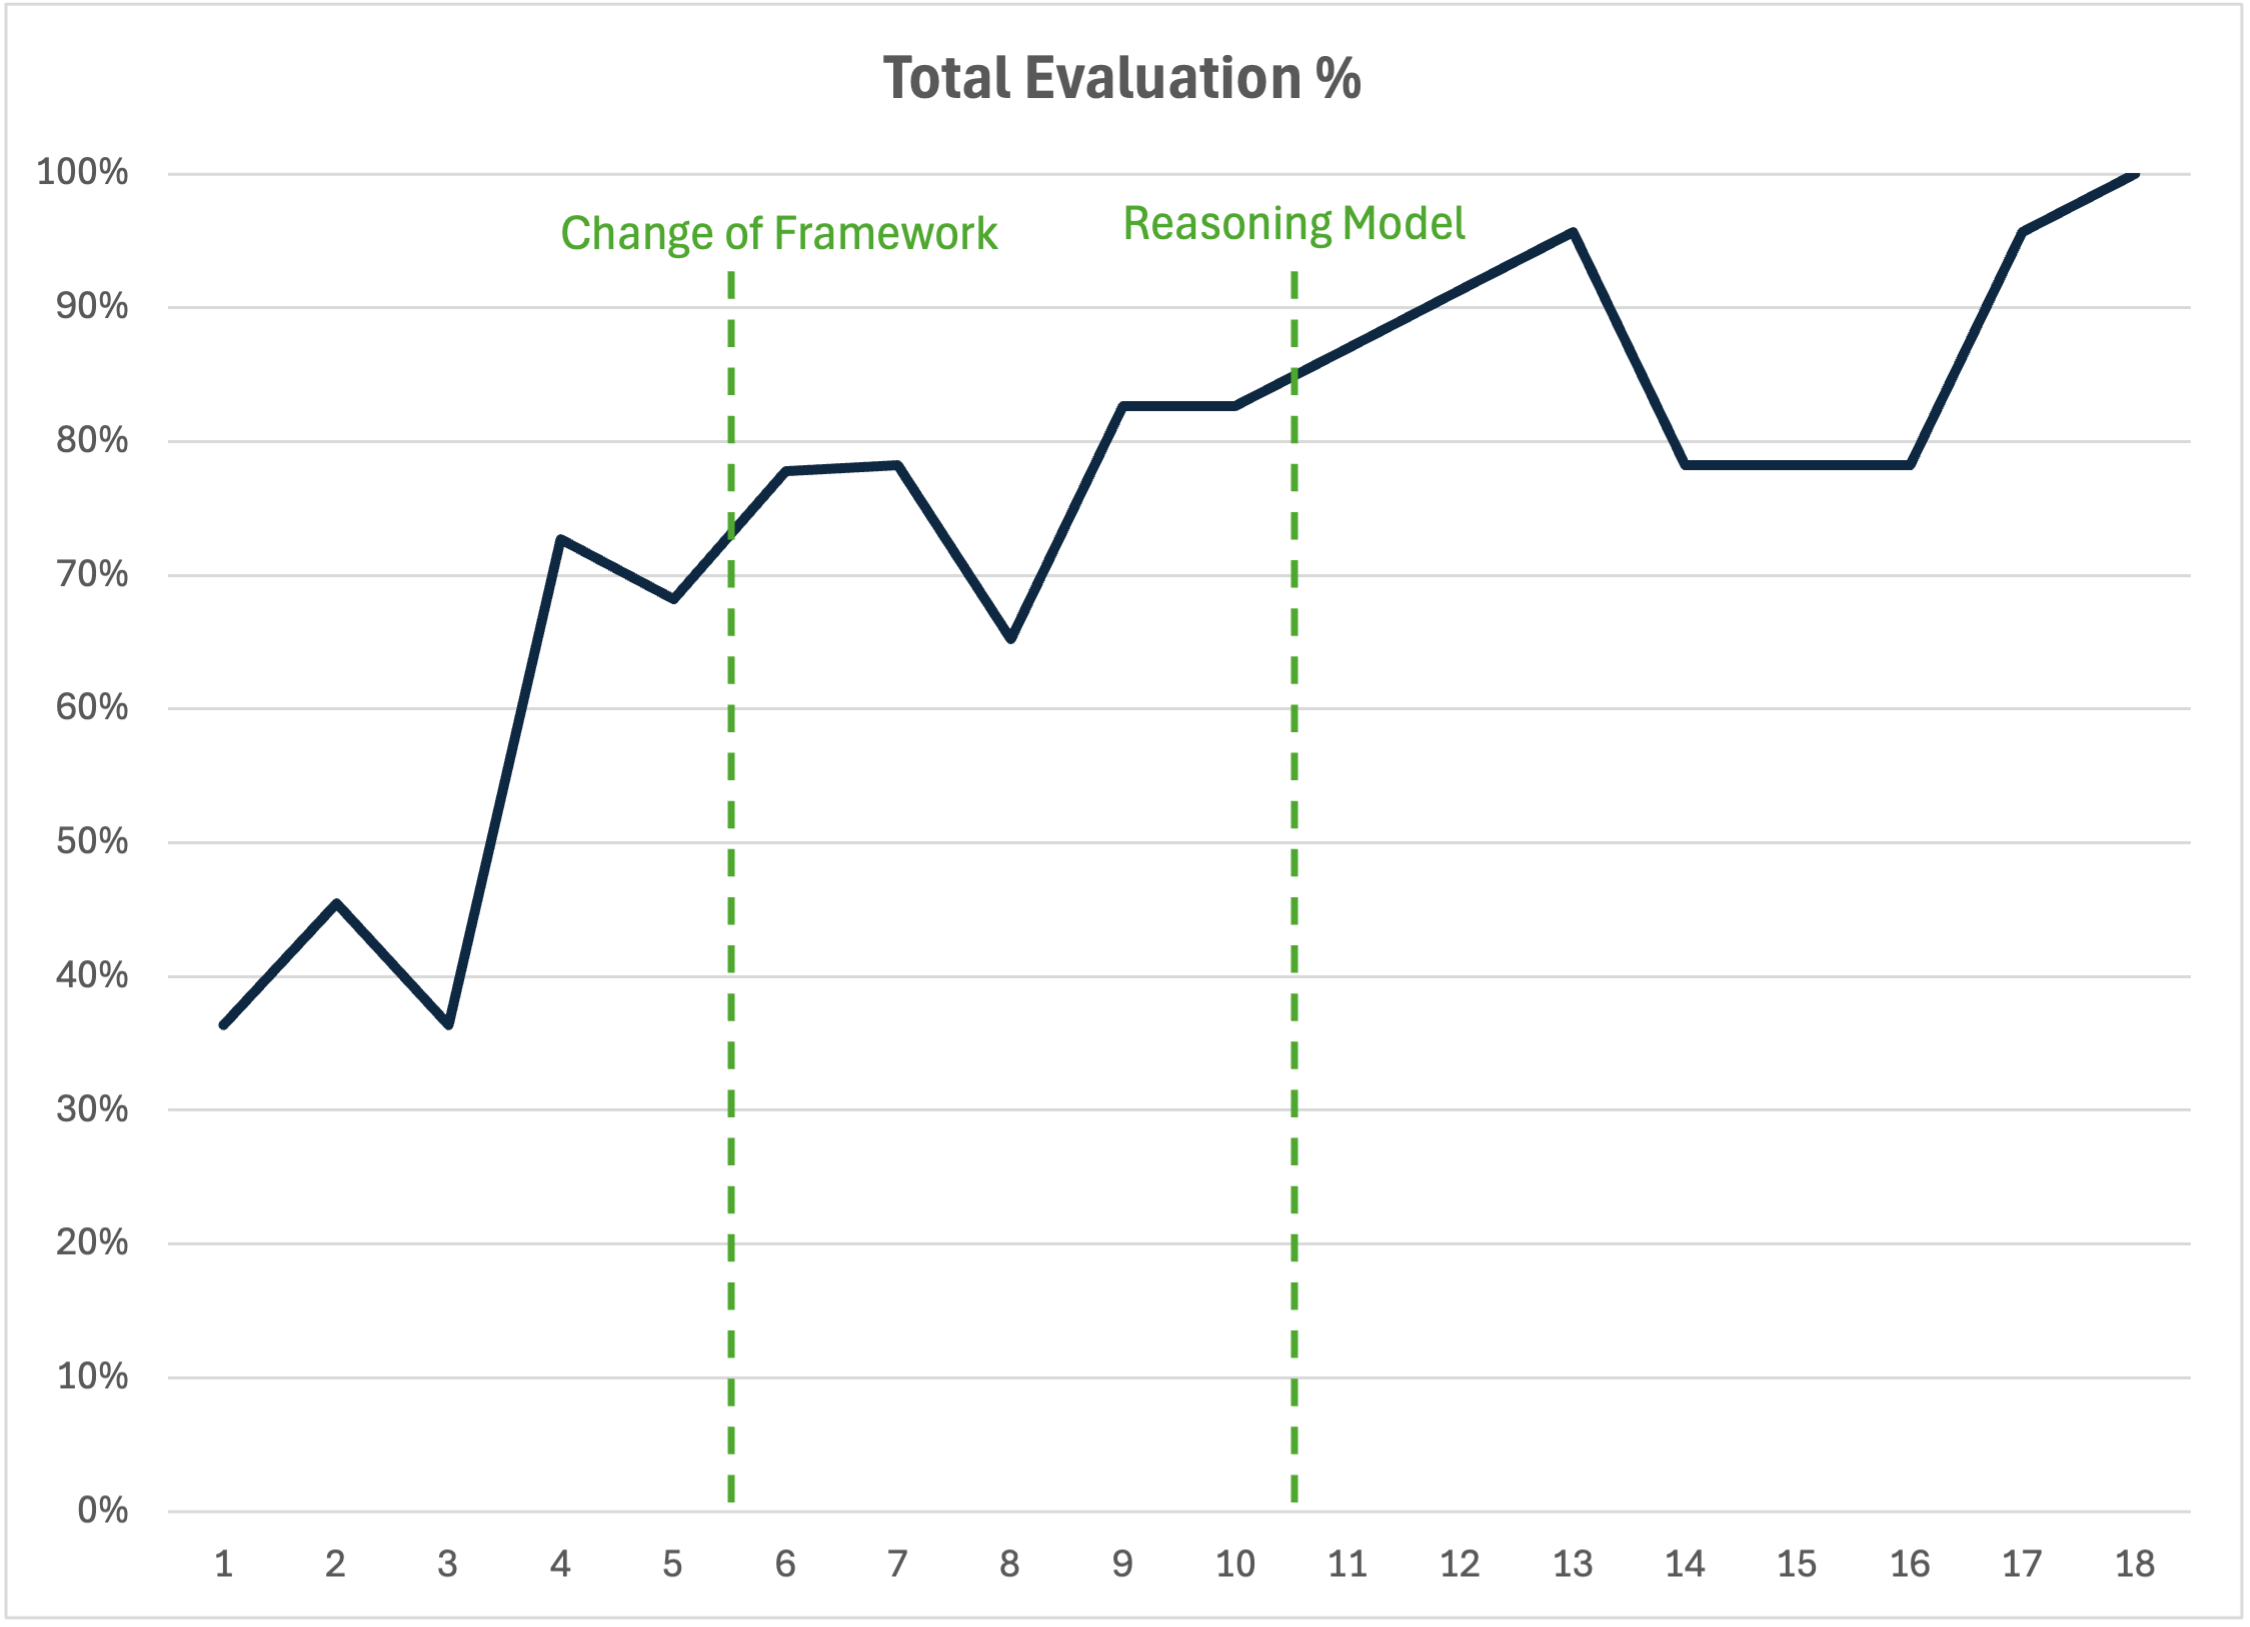
\includegraphics[width=0.61\textwidth]{images/evals-total.png}
\caption{Evolution of evaluation results}
\label{fig:evals-total}
\end{figure}

\begin{figure}[H]
\centering
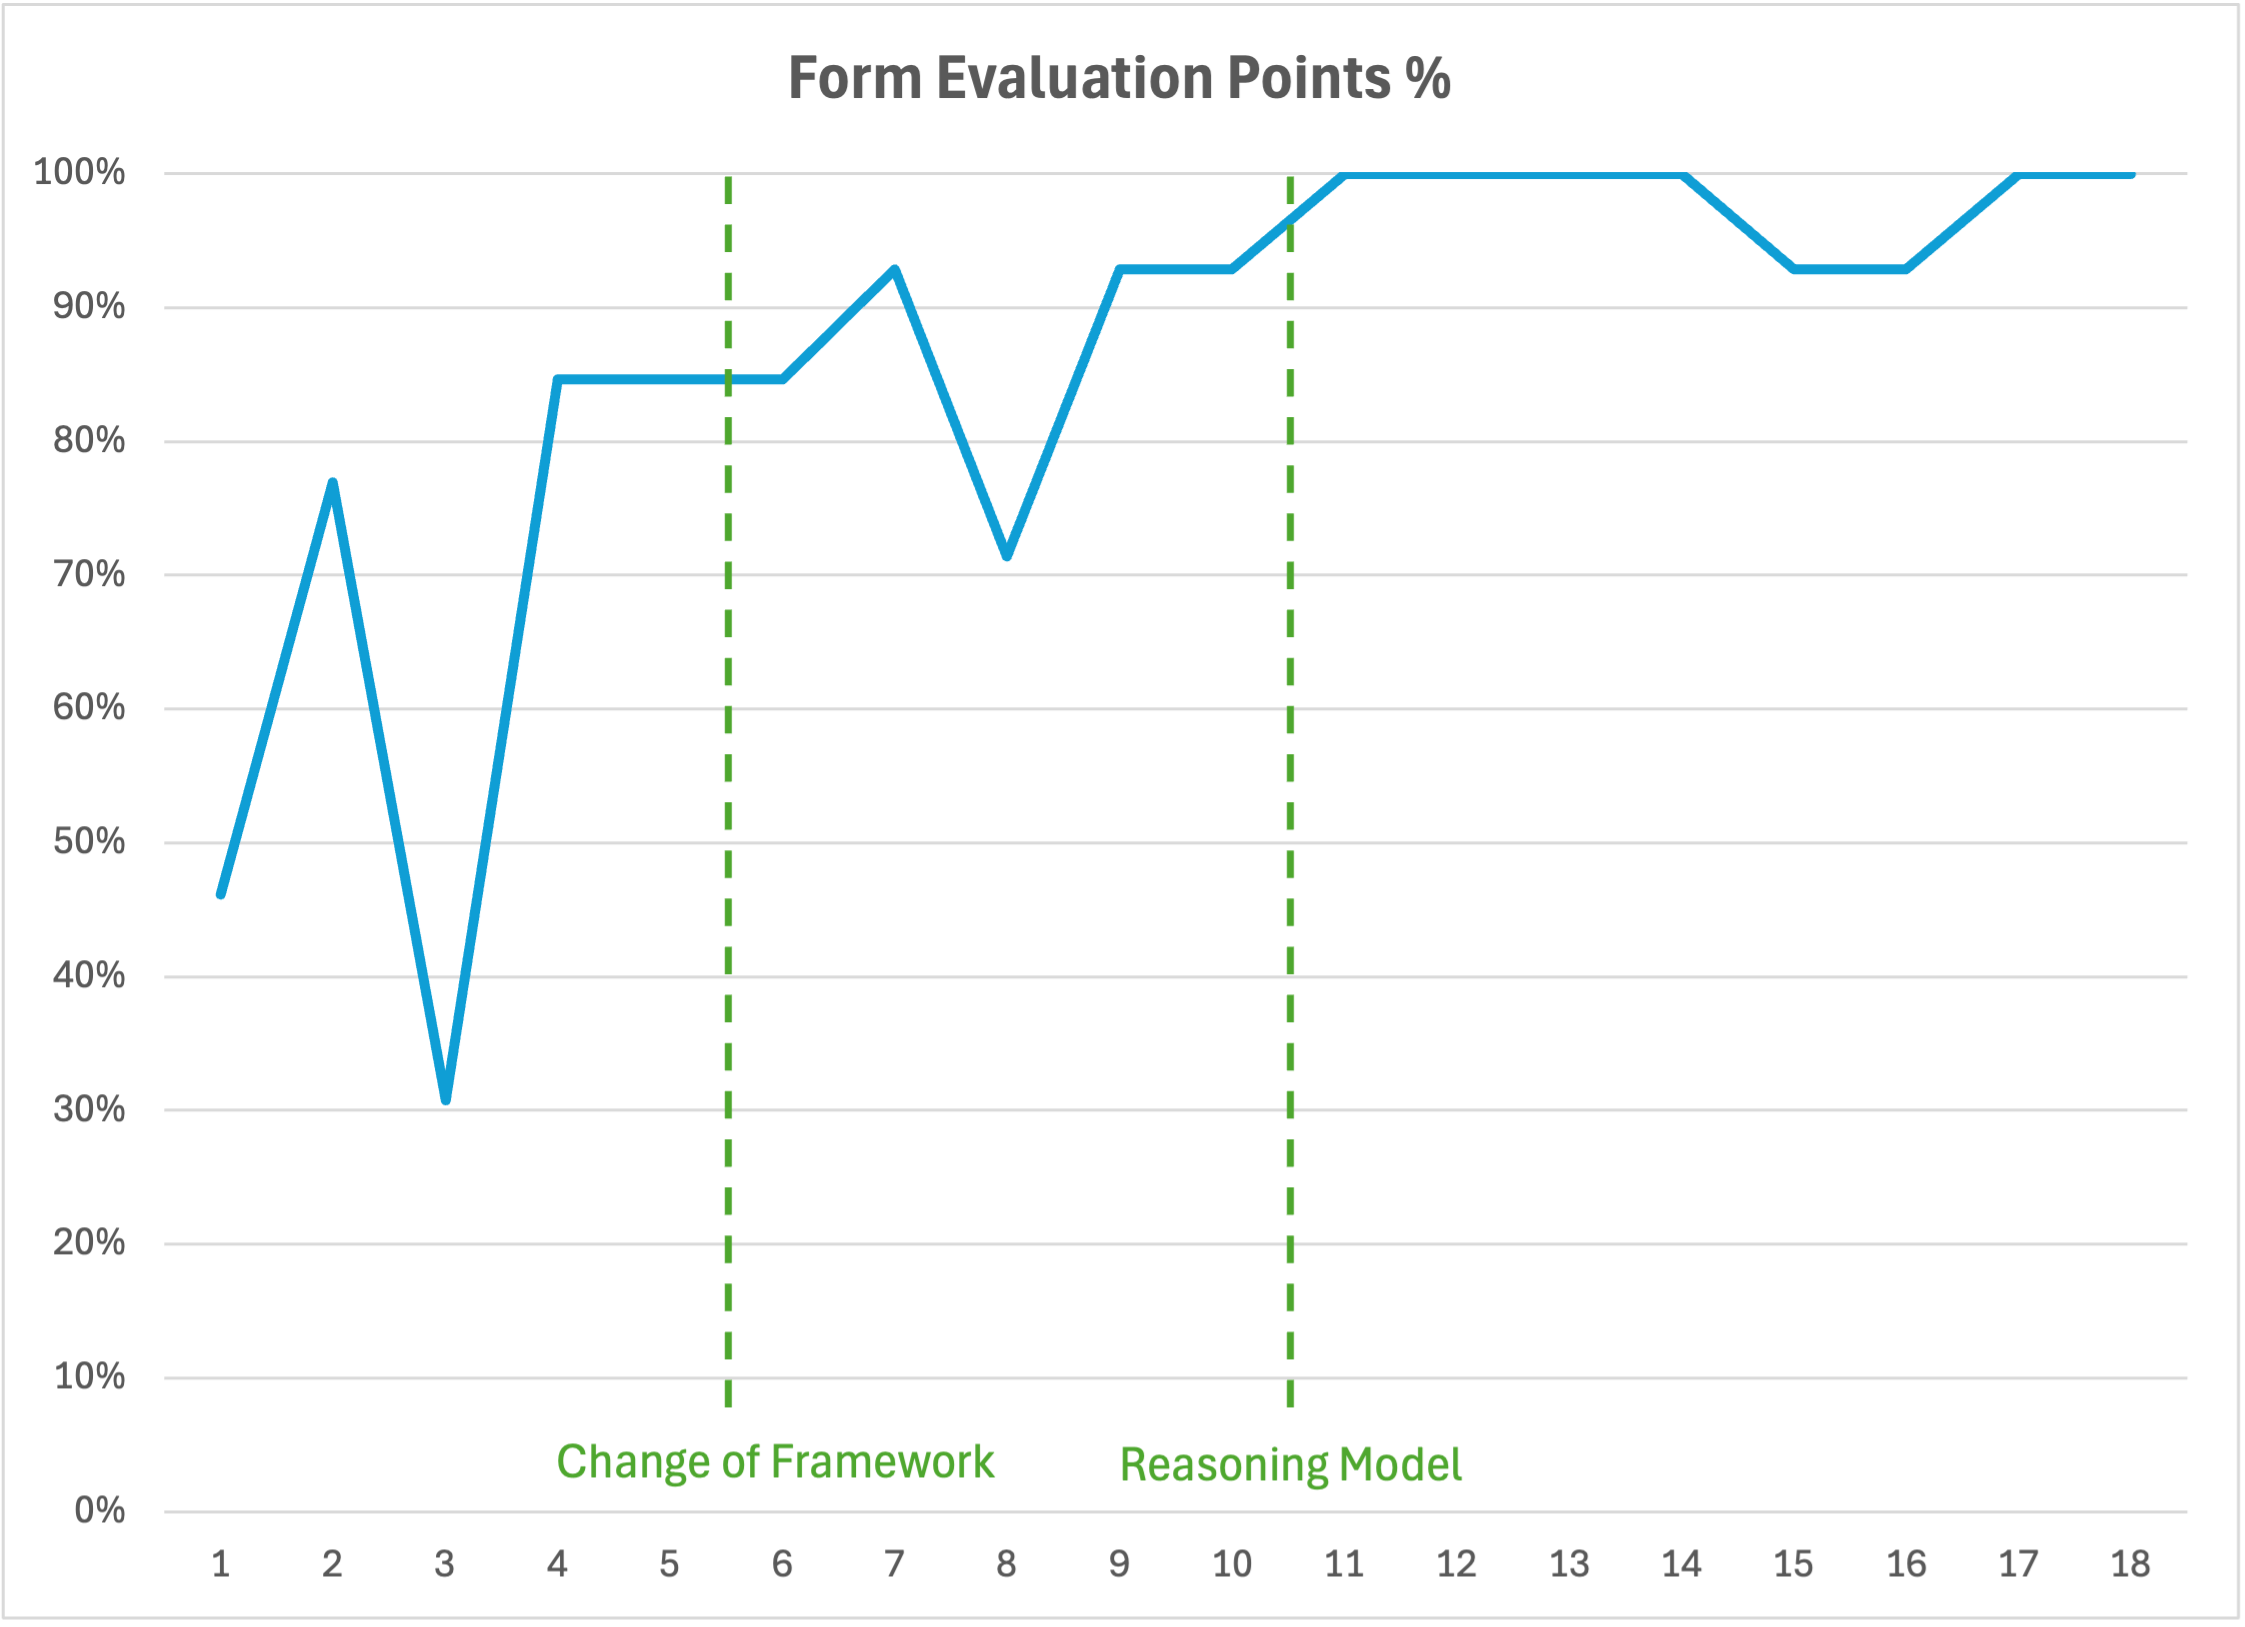
\includegraphics[width=0.61\textwidth]{images/evals-form.png}
\caption{Evolution of evaluation results considering only form items}
\label{fig:evals-form}
\end{figure}

\begin{figure}[H]
\centering
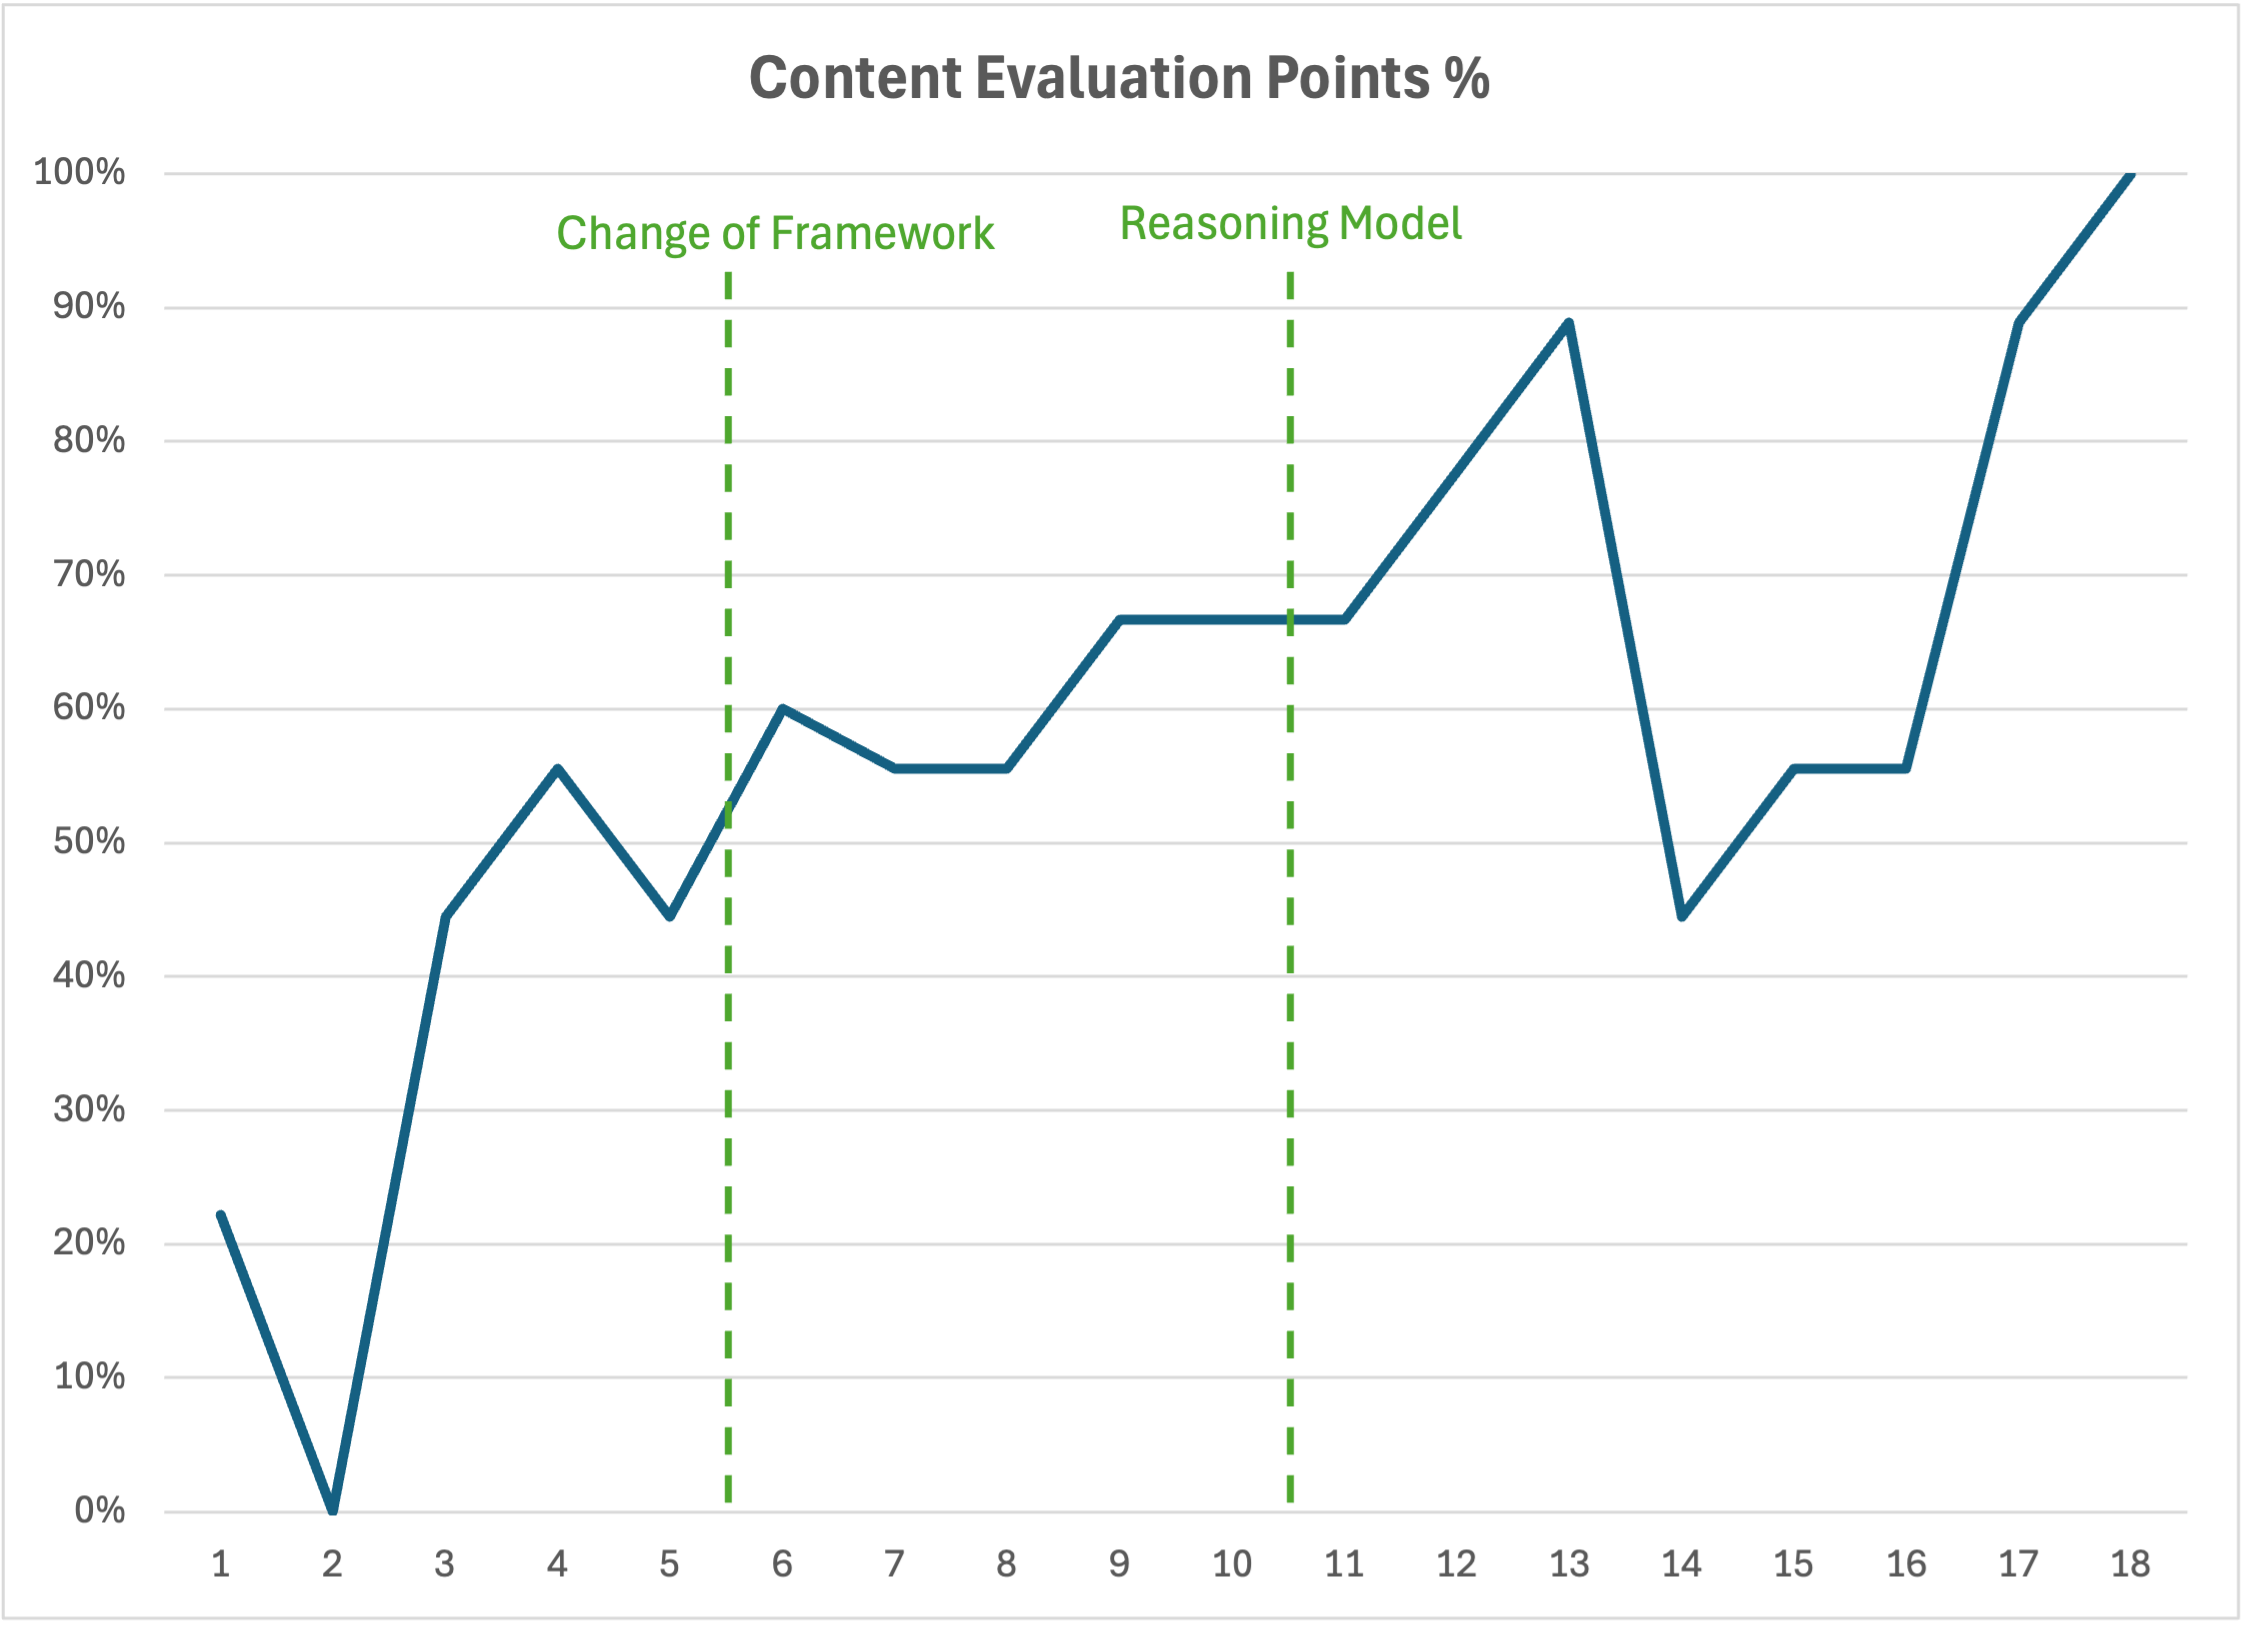
\includegraphics[width=0.61\textwidth]{images/evals-content.png}
\caption{Evolution of evaluation results considering only content items}
\label{fig:evals-content}
\end{figure}

As mentioned before, the first iteration considered a single orchestration entity, with a single task to create the entire report. As can be seen in \autoref{fig:evals-form}, this iteration could get a reasonably high score on the form evaluation, but never perfect. It consistently failed to properly present the "current" period of data --- in every case, the report analysed the entire sales history, which is not useful for a report that will be issued periodically. This is a key nuance of the task.

Moreover, as evidenced in \autoref{fig:evals-content}, this agentic architecture failed to score more than 60\% on the content score, despite changes to the task description or architecture. In fact, as can be reviewed in \autoref{fig:evals-detailed}, every iteration had issues with different parts of the content.

After an in-depth review of the intermediate steps taken by the system, the reason for this issue became clear: while iterating, the context keeps growing and growing, even if the iteration does not actually move the task forward. In this particular architecture, this growth in context also affected the context of each sub-agent, making their responses worse as the iterations progressed. This led to two insights, which drove the approach to the second iteration:

\begin{itemize}
    \item \stepcounter{kfcounter}\kfid : while LLMs can indeed perform large tasks with some success, by breaking the task into subtasks we can manage the context at each point, improving their effectiveness and reliability.
    \item \stepcounter{kfcounter}\kfid : deep research tasks increase the context quickly, but not all intermediate findings actually add information, so they benefit for summarization steps within the workflow\footnote{As opposed to most common architectures which only summarise at the end of the task}. This is in line with the findings of \cite{veseli2025positionalbiasesshiftinputs}.
\end{itemize}

The first point can be seen clearly on \autoref{fig:evals-form}. After the change to a step-by-step workflow, fluctuations in form score reduced vastly, while the content score slowly increased as the entire workflow was rebuilt. This is also highlighted by the fact that LLM steps were not reliably recommended remedy actions that were measurable; by making the recommendations part of the single deep research task, and not a separate step, the nuance is lost within the large context the task itself creates, resulting in very general recommendations.

Later on, after finishing rebuilding the workflow, the system's default model was changed to use one of OpenAI's reasoning models, leading to \stepcounter{kfcounter}\kfid : changing to a reasoning model has a smaller impact than the change to a step-by-step workflow, as the reasoning step can be approximated by the architecture of each agent within the workflow. That said, the quality of certain parts of the output, such as the graphs generated, did improve markedly by using a more powerful model.

Nevertheless, as mentioned in \autoref{chapter:design-implementation} with the change to reasoning model runs became more volatile, as reasoning models do not accept configuration variables such as Temperature, Top K or Top P. This was particularly evidenced in sub-agents that work iteratively before responding, which seemed to fall into infinite loops more easily. This led to \stepcounter{kfcounter}\kfid : autonomous agents are not guaranteed to self-recover, and the system must be planned around that. Common architectures use steps to reflect and re-plan, but this assumes that the agent will at some point finalize the task. For cases such as deep research, where there might not be clear measure for the task to be ``done'', it is important to create, and properly handle, forceful ending points.

Finally, as mentioned in \autoref{chapter:evaluation-testing} the evaluation score does not measure how useful the report is for decisions making. Some reports, for the same request and with access to the same data, might show detailed operational information by City and Product Family, while others might extract insights by Customer. All of these would get the same evaluation score, but might be more or less useful. This highlights \stepcounter{kfcounter}\kfid : at the current state of LLMs, they can be used to reduce the time spent in data extraction, but companies will still need a human in the loop to review the output, confirm whether additional information is needed, and decide how to act based on the extracted insights.

\section{Future Work}
\label{sec:future-work}

The current system is a proof of concept. As such, it can --- and should --- be improved upon to create production-ready system. The most important changes to get there would be:

\begin{enumerate}
    \item Improvements to the evaluation framework:
    \begin{itemize}
        \item Fully automate the evaluation of outputs, to allow for quicker iterations.
        \item Evaluate intermediate steps within a full execution, in addition to individually.
        \item Add objective evaluation to intermediate steps when appropriate.
    \end{itemize}
    \item Improvements to the product readiness of the user interface for configuration:
    \begin{itemize}
        \item If the system will be deployed in a publicly accessible location, add authentication.
        \item Add acceptance tests that can be run on the CI/CD pipeline.
        \item Potentially, allow different reports to run on different cron configurations.
    \end{itemize}
    \item Improvements to the agent architecture and outputs:
    \begin{itemize}
        \item Make the corrective actions proposed by the LLM when there is a ``special case" measurable, by creating a separate step in the workflow dedicated to providing and measuring the recommendations.
    \end{itemize}
\end{enumerate}

\appendix

\printbibliography

\chapter{System Manual}

\chapter{User Manual}

\chapter{Report Evaluation Questions}
\label{annex:evaluation}

\begin{table}[H]
\centering
\begin{tabular}{|p{14cm}|}
    \hline
    \textbf{Form Items} \\ \hline
    Does the report include all the required sections? \\ \hline
    Does the report actually address the required KPI? \\ \hline
    Does the report include an analysis of the evolution of the KPI? \\ \hline
    Does the report include detailed data, in addition to the high level KPI information? \\ \hline
    Does the report include at least one graph? \\ \hline
    Does the report include more than one graph? \\ \hline
    Does the report include a projection of the KPI? \\ \hline
    Is the data retrieved correct? \\ \hline
    Does the report accurately present the last information period? \\ \hline
    Is the content of the Executive Summary accurate to the section's description? \\ \hline
    Is the content of the Overview accurate to the section's description? \\ \hline
    Is the content of the Trends \& Context accurate to the section's description? \\ \hline
    Is the content of the In Depth Analysis accurate to the section's description? \\ \hline
    Is the content of the Forward Outlook accurate to the section's description? \\ \hline
\end{tabular}
\caption{Checklist of Form Items}
\end{table}


\begin{table}[H]
\centering
\begin{tabular}{|p{14cm}|}
    \hline
    \textbf{Content Items} \\ \hline
    Does the analysis in the report accurately represent the evolution of the KPI? \\ \hline
    Does the report include an analysis of the detailed data? \\ \hline
    Does the detailed analysis mention specific drivers of decline? \\ \hline
    Are all graphs relevant to the report? \\ \hline
    Are all graph types adequate for the data presented? \\ \hline
    Are all projections adequate for the data presented? \\ \hline
    Does the report accurately note any ``special case'' present? \\ \hline
    Does the report provide next steps for any ``special case'' present? \\ \hline
Are all statements in the report sustained with data? \\ \hline
\end{tabular}
\caption{Checklist of Content Items}
\end{table}

\chapter{Experiments Performed and Evaluation Results}
\label{annex:experiments}

\begin{table}[H]
\centering
\begin{tabular}{|c|c|p{7cm}|c|c|c|c|}
    \hline
    No. & Date & Notes & Default Model & Form & Content & Total \\ \hline
    1 & 02-Jul & First test with all of my MVP Agents: Magentic One (DB, Coder) + Separate Editor & gpt-4o-mini & 50\% & 29\% & 36\% \\ \hline
    2 & 02-Jul & Re run of previous experiment & gpt-4o-mini & 75\% & 29\% & 45\% \\ \hline
    3 & 03-Jul & Move Editor Agent inside team, improve quant agent prompt & gpt-4o-mini & 50\% & 29\% & 36\% \\ \hline
    4 & 04-Jul & Improve Magentic One task description & gpt-4o-mini & 75\% & 71\% & 73\% \\ \hline
    5 & 04-Jul & Improve Editor Prompt & gpt-4o-mini & 75\% & 64\% & 68\% \\ \hline
    6 & 09-Jul & First test with LangGraph --- Minimal MVP, without in-depth analysis & gpt-4o-mini & 78\% & 78\% & 78\% \\ \hline
    7 & 11-Jul & Add step for operational info just with the quant agent & gpt-4o-mini & 100\% & 64\% & 78\% \\ \hline
    8 & 15-Jul & Leave plot generation for last step & gpt-4o-mini & 67\% & 64\% & 65\% \\ \hline
    9 & 15-Jul & Re run of previous experiment  & gpt-4o-mini & 89\% & 79\% & 83\% \\ \hline
    10 & 23-Jul & Add the agent for in-depth research & gpt-4o-mini & 89\% & 79\% & 83\% \\ \hline
    11 & 24-Jul & Add the agent for in-depth research & o4-mini & 100\% & 79\% & 87\% \\ \hline
    12 & 28-Jul & Change prompt: `concise' to `detailed' & o4-mini & 100\% & 86\% & 91\% \\ \hline
    13 & 28-Jul & Re run of previous experiment & o4-mini & 100\% & 93\% & 96\% \\ \hline
    14 & 29-Jul & Add capacity for report writing graph to load csv files & o4-mini & 100\% & 64\% & 78\% \\ \hline
    15 & 29-Jul & Re run of previous experiment & o4-mini & 89\% & 71\% & 78\% \\ \hline
    16 & 30-Jul & Add check for coding agent intermediate input vs final input & o4-mini & 89\% & 71\% & 78\% \\ \hline
    17 & 30-Jul & Update prompt in quant agent to reduce intermediate requests for user input & o4-mini & 100\% & 93\% & 96\% \\ \hline
    18 & 31-Jul & Update prompt in internal data agent to ensure all files are generated in the right folder & o4-mini & 100\% & 100\% & 100\% \\ \hline
    \end{tabular}
\caption{Experiments performed with Evaluation scores}
\end{table}

\begin{sidewaysfigure}
    \centering
    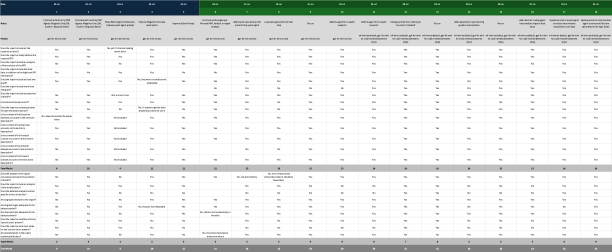
\includegraphics[width=\textheight]{images/evals-detail.png}
    \caption{Detailed evaluation scores; empty cells are items that do not apply to that specific experiment.}
    \label{fig:evals-detailed}
\end{sidewaysfigure}

\chapter{Sample Automated Evaluation}
\label{annex:sample-eval}

\begin{verbatim}
async def test_file_creation(quantitative_agent):
    """
    Test the agent creates at least one file in the temp directory.
    """

    query = f"""The company's sales for the last three years are as follows:' 
    
    {california_monthly_sales_in_db}
    
    Perform a detailed analysis of the sales data, including trends, patterns, and insights."""

    response = await quantitative_agent.ainvoke(messages=[HumanMessage(content=query)])
    response_content = extract_graph_response_content(response)

    from src.agents.utils.output_utils import get_all_files_mentioned_in_response

    files_mentioned = get_all_files_mentioned_in_response(response_content)
    try:
        # Assert that there is at least one file created in the temp directory
        assert len(files_mentioned) > 0, "No files were created in the temp directory."
        # Assert all files are csv files
        assert all(file.endswith(".csv") for file in files_mentioned), (
            "Not all created files are CSV files."
        )
        # Assert that the file actually exists
        for file_name in files_mentioned:
            file_path = test_temp_dir / file_name
            assert file_path.exists(), f"File {file_name} does not exist at {file_path}"
    finally:
        # Clean up the temp directory after the test
        for file in files_mentioned:
            file_path = test_temp_dir / file
            file_path.unlink(missing_ok=True)
\end{verbatim}

\chapter{Automated Testing Suite Results}
\label{annex:test-results}

The following are the results of the last run of the testing suite. Please note the interpretation of failed tests mentioned on \autoref{sec:components-evals}.

\begin{figure}[H]
\centering
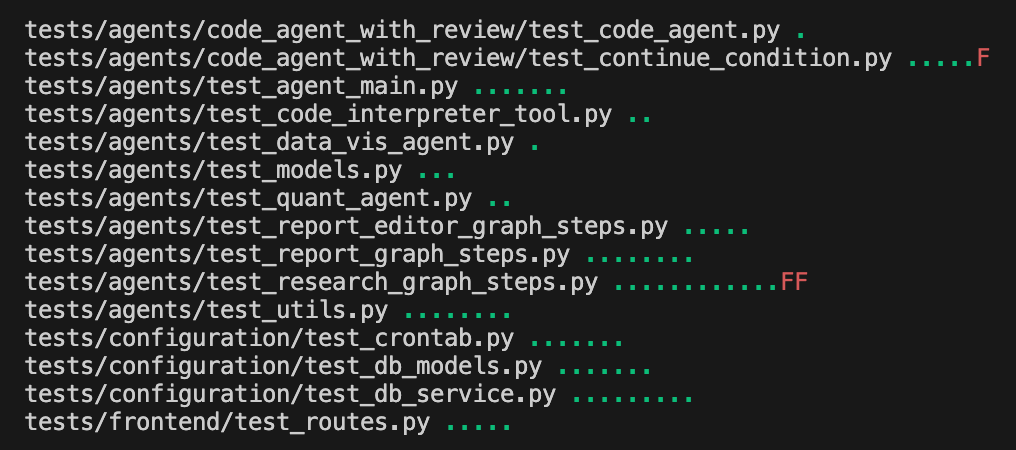
\includegraphics[width=0.61\textwidth]{images/test-results.png}
\caption{Test results by test file}
\end{figure}

\begin{figure}[H]
\centering
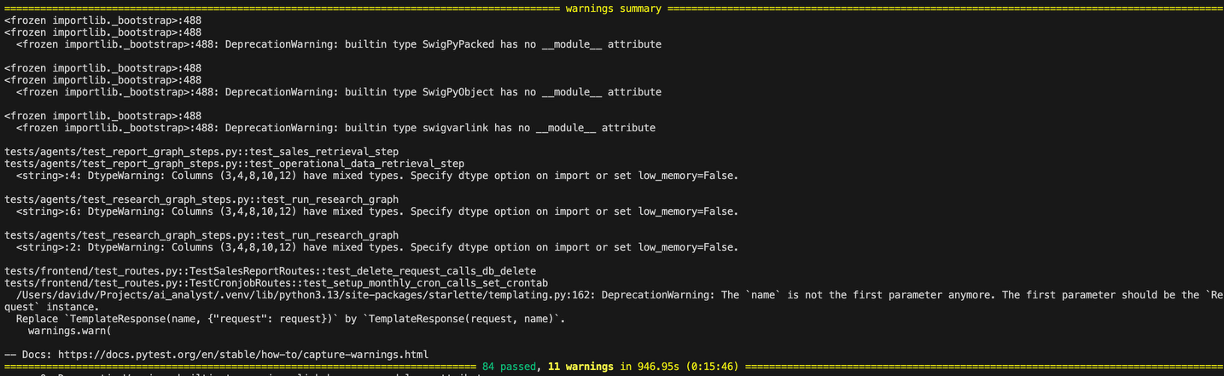
\includegraphics[width=1\textwidth]{images/test-results-bottom.png}
\caption{Test results summary and failures}
\label{fig:evals-form}
\end{figure}

\begin{figure}[H]
\centering
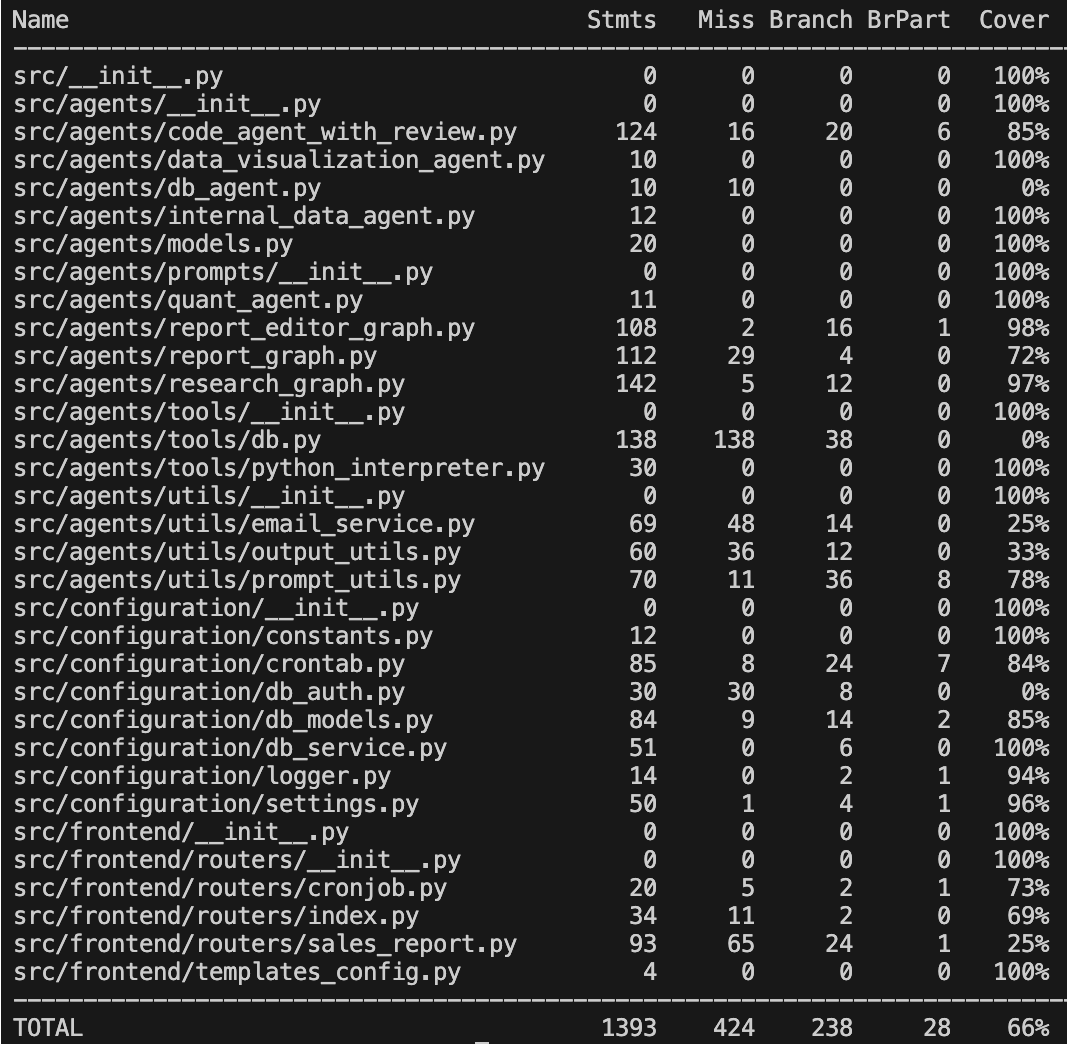
\includegraphics[width=0.61\textwidth]{images/test-coverage.png}
\caption{Test coverage output}
\label{fig:evals-form}
\end{figure}

\chapter{Generated Report --- Sample}

\end{document}